
\documentclass{article} % For LaTeX2e

\PassOptionsToPackage{table}{xcolor}
\usepackage{iclr2027_conference,times}


% Optional math commands from https://github.com/goodfeli/dlbook_notation.
\input{math_commands.tex}

\usepackage{hyperref}
\usepackage{url}
\usepackage{graphicx}
\usepackage{amsthm,needspace}
\usepackage{booktabs,tabularx,multirow,placeins}
\usepackage[table]{xcolor}
\usepackage[most]{tcolorbox}
\newtheorem{lemma}{Lemma}[section]
\newtheorem{theorem}{theorem}[section]

% Shared styling for the distribution-matching tables.
\definecolor{frameworkink}{RGB}{38,57,76}
\definecolor{frameworktint}{RGB}{241,245,249}
\definecolor{frameworkforward}{HTML}{0072B2}
\definecolor{frameworkreverse}{HTML}{B45309}
\definecolor{frameworkpolicy}{HTML}{8E4585}
\newcommand{\forwardKL}{\textcolor{frameworkforward}{Forward KL}}
\newcommand{\reverseKL}{\textcolor{frameworkreverse}{Reverse KL}}
\newcommand{\targetpolicy}{\textcolor{frameworkpolicy}{\pi_\theta}}
\newcommand{\algorithmgroup}[1]{%
  % Add space outside the rules while keeping the heading row height fixed.
  \specialrule{\lightrulewidth}{2pt}{0pt}%
  \multicolumn{4}{l}{\textcolor{frameworkink}{\textbf{#1}}}\\%
  \specialrule{\lightrulewidth}{0pt}{2pt}}

% Reusable summary box: \begin{takeaway} ... \end{takeaway}.
\definecolor{takeawayaccent}{HTML}{3D647A}
\definecolor{takeawaybackground}{HTML}{F1F5F8}
\newtcolorbox{takeaway}{
  enhanced,
  colback=takeawaybackground,
  coltext=black,
  frame hidden,
  borderline west={1.5pt}{0pt}{takeawayaccent},
  sharp corners,
  boxrule=0pt,
  boxsep=0pt,
  left=10pt, right=10pt, top=8pt, bottom=8pt,
  before skip=10pt, after skip=10pt,
  fontupper=\normalfont\small,
  halign=left,
  before upper={\textcolor{takeawayaccent}{\bfseries Takeaway.}\enspace},
}

% Reusable main-idea box: \begin{insight} ... \end{insight}.
\definecolor{insightaccent}{HTML}{B45309}
\definecolor{insightbackground}{HTML}{FFF5E8}
\newtcolorbox{insight}{
  enhanced,
  colback=insightbackground,
  coltext=black,
  frame hidden,
  borderline west={1.5pt}{0pt}{insightaccent},
  sharp corners,
  boxrule=0pt,
  boxsep=0pt,
  left=10pt, right=10pt, top=8pt, bottom=8pt,
  before skip=10pt, after skip=10pt,
  fontupper=\normalfont\small,
  halign=left,
  before upper={\textcolor{insightaccent}{\bfseries Insight.}\enspace},
}


\title{A Distribution-Matching Perspective on LLM Training Algorithms}

% Authors must not appear in the submitted version. They should be hidden
% as long as the \iclrfinalcopy macro remains commented out below.
% Non-anonymous submissions will be rejected without review.

\author{Antiquus S.~Hippocampus, Natalia Cerebro \& Amelie P. Amygdale \thanks{ Use footnote for providing further information
about author (webpage, alternative address)---\emph{not} for acknowledging
funding agencies.  Funding acknowledgements go at the end of the paper.} \\
Department of Computer Science\\
Cranberry-Lemon University\\
Pittsburgh, PA 15213, USA \\
\texttt{\{hippo,brain,jen\}@cs.cranberry-lemon.edu} \\
\And
Ji Q. Ren \& Yevgeny LeNet \\
Department of Computational Neuroscience \\
University of the Witwatersrand \\
Joburg, South Africa \\
\texttt{\{robot,net\}@wits.ac.za} \\
\AND
Coauthor \\
Affiliation \\
Address \\
\texttt{email}
}

% The \author macro works with any number of authors. There are two commands
% used to separate the names and addresses of multiple authors: \And and \AND.
%
% Using \And between authors leaves it to \LaTeX{} to determine where to break
% the lines. Using \AND forces a linebreak at that point. So, if \LaTeX{}
% puts 3 of 4 authors names on the first line, and the last on the second
% line, try using \AND instead of \And before the third author name.

\newcommand{\fix}{\marginpar{FIX}}
\newcommand{\new}{\marginpar{NEW}}

%\iclrfinalcopy % Uncomment for camera-ready version, but NOT for submission.
\begin{document}


\maketitle

\begin{abstract}
In this work, we propose a unified framework for training algorithms across different stages of modern large language model development, based on the perspective of distribution matching. We show that a broad class of language model training algorithms can be interpreted as minimizing a certain divergence between the current model and a target distribution, and that characterizing the properties of this target distribution provides substantial insight into the behavior of the corresponding training algorithms.
By analyzing specific forms of the target distribution, we establish that On-Policy Distillation (OPD) enjoys an advantage over classical Knowledge Distillation (KD) when the current model distribution is close to the target distribution, while exhibiting a disadvantage when the two distributions are far apart. Furthermore, when the target distribution itself depends on the model being optimized, we show that the accumulation estimation variance can induce a deterministic degradation of the target distribution.
These results provide a theoretical explanation, at least in part, for the long-term behavior of existing Reinforcement Learning (RL) algorithms, and further study suggest several principled and reliable approaches for mitigating the associated degradation. We believe that this theoretical perspective can deepen the research community's understanding of language model training algorithms and provide useful guidance for future research.
\end{abstract}

\section{Introduction}

Modern Large Language Models (LLMs) require a complex training pipeline with different algorithms from pre-training to post-training~\citep{team_kimi_2026, deepseek-ai_deepseek-v4_2026, glm-5-team_glm-5_2026}. These algorithms are motivated by different intuitions. For example, the objectives of pre-training and Supervised Fine-Tuning (SFT) arise directly from distribution matching under the cross-entropy loss; On Policy Distillation (OPD) is constructed around on-policy sampling~\citep{lochab_uniform-correct_2026}; Reinforcement Learning (RL) aims to maximize the expected reward~\citep{williams_simple_1992}; and MaxRL can be viewed as arising from maximum-likelihood estimation of correct solutions~\citep{tajwar_maximum_2026}. Our goal is to develop a unified characterization of these seemingly different algorithms in the context of language models. Such a unified perspective may help disentangle the complexity underlying these methods, facilitate the theoretical study of their properties, and provide new insights into their connections and behavior.

Many of the training algorithms of LLMs already admit a distribution matching interpretation~\citep{korbak_reinforcement_2022, khalifa_distributional_2021}, whereas RL is often viewed fundamentally distinct. In this work we first studied the property of an ideal update step in RL and show that, under binary rewards, it preserves the conditional distribution associated with a given reward value. Moreover, if we consider the forward KL divergence between the current model and this conditional distribution, the resulting training direction coincides with that of RL on a fixed sample. Similar results can also be extended to RL with nonbinary rewards.

This provides a unified perspective that places the mainstream training algorithms for LLMs within a common distribution-matching framework. Analyzing how the target distribution changes and affects the learning dynamics under different conditions can yield a variety of interesting theoretical results that characterize the properties of these algorithms.

Depending on whether the target distribution being optimized depends on the current model distribution or not, these algorithms can be further categorized into iterative and non-iterative methods. In what follows, we progressively examine the properties of three classes of algorithms, from simpler to more complex cases: non-iterative methods, iterative methods with zero-mean gradients, and iterative methods with nonzero-mean gradients.

For the first class, we mainly study OPD and SFT-based classical Knowledge Distillation ~\citep{hinton_distilling_2015} algorithms. By analyzing the variance induced by different target distributions under different assumptions, we roughly classified the boundary of effectiveness of these algorithms, providing a theoretical explanation for previous empirical observations regarding the stability of distillation algorithms~\citep{li_rethinking_2026, oh_kl_2026}.

The second class primarily consists of the iterative self-distillation and reversed iterative self-distillation algorithms that we introduce. These methods lie between distillation and RL, while retaining theoretical properties that are more amenable to analysis. Within this class, we identify an intriguing \emph{variance accumulation} phenomenon in iterative training, which leads to a monotonic decrease in the expected entropy of the target distribution. In contrast to previous local results derived from training dynamics~\citep{cui_entropy_2025, ren_learning_2025, jin_revisiting_2026}, our analysis further shows that, although the model entropy may either increase or decrease after an individual update, its long-term behavior exhibits a systematic downward trend under the variance accumulation.

The third class mainly consists of RL and MaxRL. We first provide further empirical evidence that variance accumulation affects entropy in RL-type algorithms, and then analyze the deterministic bias induced by the geometric properties of the model parameterization. Based on these observations, we derive several principled algorithmic corrections, which may also provide useful guidance for the development of future training algorithms. In realistic training settings, however, the target distribution invariance of RL and MaxRL under idealized conditions is no longer preserved. Their target distributions instead exhibit collapse, driven in part by effects such as variance accumulation. Such target distribution drift serves as an important manifestation of the discrepancy between practical training dynamics and their idealized counterparts, offering new insights into the sources of this discrepancy and potential directions for algorithmic improvement.

%In this work we find that all these algorithms can be naturally interpreted as minimizing the divergence between the current model and a target distribution either explicitly or implicitly. Analyzing how the target distribution changes and affects the learning dynamics under different conditions can yield a variety of interesting theoretical results that characterize the properties of these algorithms.

% These algorithms can be further classified into two categories. We call an algorithm iterative if the target distribution depends on the current model distribution, and noniterative otherwise. We primarily studied three different settings from simple to complex.

% \subsection{Noniterative Methods}
%
% We begin by studying distillation methods with a fixed target distribution.
% %Here "noniterative" means that the target distribution is not updated through training steps.
% We find that under the \emph{proximal limit}, where the student model coincides with the target, both forward Knowledge Distillation (KD) and OPD objective has zero mean. We can further prove that OPD has zero variance at the proximal limit while the variance of KD is nonzero. The variance analysis further indicates that the estimation error of OPD is strictly lower than that of KD when the student distribution is close to the teacher. This provides a theoretical guarantee of the effectiveness boundary of these methods, that OPD should be more performant than KD in the proximal case, while being less performant in the distal regime.
%
% \subsection{Iterative Methods with Zero Mean Gradients}
%
% Nonzero gradient-estimation variance at the proximal limit has further consequences for iterative methods, in which the target distribution depends on the current policy. Our analysis shows that ideal updates in distribution space preserve the target distribution in self-distillation and binary-reward RL. In practice, however, gradient-estimation noise can cause the target distribution to drift after each training step. Under local concavity conditions, we show that this \emph{variance accumulation} causes expected entropy to decrease over training, providing a possible mechanism for entropy collapse. Entropy dynamics have been widely studied in RL, with many existing analyses focusing on individual updates~\citep{cui_entropy_2025, jin_revisiting_2026, wang_entropy_2026}. Our analysis extends this perspective to the effects of repeated updates and offers an explanation for long-term behavior.
%
% We design iterative self-distillation and reversed iterative self-distillation experiments to examine the effects of variance accumulation, and observe counter-intuitive results consistent with our theoretical predictions.
%
% \subsection{Iterative Methods with Nonzero Mean Gradients}
%
% RL is a representative iterative distribution-matching method with a nonzero mean gradient. We first show that, when the failure-conditioned distribution has at least as much entropy as the success-conditioned distribution, the target has lower entropy than the current policy. This provides a natural source of entropy reduction during RL training. Such a reduction does not necessarily imply the loss of diversity among correct responses observed in previous work~\citep{yue_does_2025, tajwar_maximum_2026, jin_revisiting_2026}. Our focus is on the deterioration of the target distribution itself, which can arise from both variance accumulation and geometric bias induced by the model parameterization. We conduct experiments to assess the effects of variance on RL algorithms and derive a correction to standard RL through an analysis of this geometric bias. The correction exhibits advantages over standard Group Relative Policy Optimization (GRPO).

% \subsection{Summary of Contributions}

Our contributions are threefold:

\begin{itemize}
\item We introduce a unified theoretical framework that interprets learning algorithms across the LLM training pipeline through distribution matching. By focusing on target distributions and their evolution, this framework clarifies the connections between algorithms and provides a systematic approach to analyzing their properties.
\item We theoretically characterize the regimes in which OPD and SFT have lower gradient-estimation variance, through analysis at the proximal limit and under specified conditions in the distal regime. These results can guide the application of distillation methods and inform future algorithm design.
\item We identify variance accumulation and geometric bias as mechanisms that can drive target-distribution drift and reduce diversity in iterative RL. This analysis motivates a bias correction for RL and suggests directions for future research.
\end{itemize}


\section{A Unified Framework of LLM Training Algorithms}

\subsection{Pre-Training And Distillation Algorithms}

In pre-training and Supervised Fine-Tuning (SFT), minimizing the standard
cross-entropy loss is equivalent to minimizing the forward KL divergence
from the data distribution to the model distribution.
To make this precise, let $\mathcal{D}=\{x^{(i)}\}_{i=1}^N$ be a fixed,
nonempty dataset of token sequences, let
$p_{\mathcal{D}}(x)=N^{-1}\sum_{i=1}^N\mathbf{1}\{x^{(i)}=x\}$ be its
empirical distribution, and let $\pi_\theta(x)$ be the model probability
of sequence $x$ with parameter $\theta$. Then

\begin{align}
 D_{\mathrm{KL}}(p_{\mathcal{D}}\Vert\pi_\theta)
 &= \mathbb{E}_{x\sim p_{\mathcal{D}}}
    \left[\log\frac{p_{\mathcal{D}}(x)}{\pi_\theta(x)}\right] \notag = -\mathbb{E}_{x\sim p_{\mathcal{D}}}[\log\pi_\theta(x)]
    -H(p_{\mathcal{D}}) \notag\\
 &= \mathcal{L}_{\mathrm{CE}}(\theta)-H(p_{\mathcal{D}}),
 \label{eq:ce-forward-kl}
\end{align}

Here the empirical cross-entropy loss is
$\mathcal{L}_{\mathrm{CE}}(\theta)=-N^{-1}\sum_{i=1}^N
\log\pi_\theta(x^{(i)})$.
The data entropy $H(p_{\mathcal{D}})=-\mathbb{E}_{x\sim p_{\mathcal{D}}}
[\log p_{\mathcal{D}}(x)]$ is finite and independent of $\theta$ which has no effect on the gradient. This proves the equivalence.

For SFT, let $x$ denote a prompt and $y$ its target response, with fixed
empirical joint distribution $p_{\mathcal{D}}(x,y)$. The same decomposition
holds conditionally:

\begin{align}
  \mathcal{L}_{\mathrm{SFT}}(\theta) &= 
  -\mathbb{E}_{(x,y)\sim p_{\mathcal{D}}}
  [\log\pi_\theta(y\mid x)]\\
  &=\mathbb{E}_{x\sim p_{\mathcal{D}}}
 \left[D_{\mathrm{KL}}\bigl(p_{\mathcal{D}}(\cdot\mid x)
 \Vert\pi_\theta(\cdot\mid x)\bigr)\right]
 +H_{p_{\mathcal{D}}}(Y\mid X),
 \label{eq:sft-conditional-kl}
\end{align}

Under the autoregressive factorization,
$-\log\pi_\theta(y\mid c)=-\sum_{t=1}^{|y|}
\log\pi_\theta(y_t\mid c,y_{<t})$, this sequence-level objective is exactly the sum of token-level
cross-entropies with ground-truth prefixes.

In many applications the response could come from a teacher model $\pi_t$, instead of the dataset. Then the training objective of SFT would become minimizing the forward KL divergence between the teacher model and the student model. This yields the classical SFT-based Knowledge-Distillation (KD) algorithm~\citep{hinton_distilling_2015}, which is often simply called SFT as well:

\begin{align}
  \mathcal{J}_{\mathrm{KD}} &= -\mathbb{E}_{x\sim\mathcal{D}} [D_{\mathrm{KL}}\bigl(\pi_t (\cdot\mid x)\Vert \pi_\theta (\cdot\mid x)\bigr)] = \mathbb{E}_{x\sim\mathcal{D}, y\sim\pi_t (\cdot\mid x)} [\log \pi_\theta (y\mid x)] - H(\pi_t).
  \label{eq:kl-loss}
\end{align}

OPD recently emerged as a new algorithm for distillation tasks~\citep{thinking_machines_lab_-policy_2025}. It can exhibit superior performance than SFT in some cases, and received great attention from the industry~\citep{team_kimi_2026, deepseek-ai_deepseek-v4_2026, glm-5-team_glm-5_2026}. While in some cases this algorithm may also be unstable and failed to complete the distillation task~\citep{li_rethinking_2026}. The key difference between OPD and KD is that, OPD uses sequence-level reverse KL divergence as the training objective:

\begin{align}
  \mathcal{J}_{\mathrm{OPD}} &= -\mathbb{E}_{x\sim\mathcal{D}} [D_{\mathrm{KL}}\bigl(\pi_\theta (\cdot\mid x)\Vert \pi_t (\cdot\mid x)\bigr)]
  = \mathbb{E}_{x\sim\mathcal{D}, y\sim\pi_\theta (\cdot\mid x)} [\log \frac{\pi_t (y\mid x)}{\pi_\theta (y\mid x)}].
  \label{eq:opd-loss}
\end{align}

The on policy nature of OPD directly come from the requirement of reverse KL divergence. As the expectation of reverse KL is calculated under the student distribution, we should use the student to generate samples. We should note that the sequence-level KL objective directly yields sampled-token OPD. While there exist several variants of this OPD~\citep{li_rethinking_2026}, this sampled-token OPD is indeed adopted by the industry~\citep{team_kimi_2026} and share some important properties with other variants. the following analysis will primarily be built upon this algorithm.

\subsection{Reinforce Learning Algorithms}

All the algorithms methoned above has a clear definition of the target distribution. However, as another central component of post-training, Reinforcement Learning (RL) is not defined by such divergence. The objective of RL is to maximize the expected reward $r$ given to each possible action of the policy model, while for LLMs this action is typically a sequence generation. Its standard objective and gradient are~\citep{williams_simple_1992}:

\begin{equation}
  \mathcal{J}_{\mathrm{RL}} = \mathbb{E}_{x\sim\mathcal{D}, y\sim\pi_\theta (\cdot\mid x)} [r(x, y)],\qquad \nabla_\theta \mathcal{J}_{\mathrm{RL}} = \mathbb{E}_{x\sim\mathcal{D}, y\sim\pi_\theta (\cdot\mid x)} [r(x, y) \nabla_\theta \log \pi_\theta].
  \label{eq:std-rfalgo}
\end{equation}

% In this work we will show that RL algorithms can also be expressed in the form of distribution matching objective under 0-1 reward, and the analysis on the target distribution can further reveal some interesting properties of these algorithms.

In fact, this objective also implicitly introduces a target distribution. We first characterize an ideal policy update that improves expected reward
while remaining close to the current policy under a forward-KL restriction. (Similar result also holds for reverse-KL restriction)

\begin{theorem}[Reward reweighting under a forward-KL restriction]
\label{lem:reward-reweighting}
For a prompt $x$, the ideal update maximizing
$\mathbb E_{y\sim q}[r(x,y)]-\beta D_{\mathrm{KL}}(\pi_\theta\Vert q)$
over response distributions $q$, with KL penalty $\beta>0$, is
\begin{equation}
 q^*(y\mid x)
 =\frac{\beta\pi_\theta(y\mid x)}{\lambda_x-r(x,y)},
 \label{eq:reward-reciprocal-tilt}
\end{equation}
where $\lambda_x$ normalizes the distribution. Responses with the same
reward receive the same probability multiplier, preserving their
conditional distribution.
\end{theorem}
\noindent\hyperref[app:reward-reweighting]{Proof: Appendix~\ref*{app:reward-reweighting}.}

Under binary rewards, we can verify that this update preserves the success-conditioned distribution
$\pi_\theta^+(\cdot\mid x)
=\pi_\theta(\cdot\mid x,r(x,y)=1)$. If we use this distribution as the training target, matching
this conditional distribution with the forward KL gives the following identity.

\Needspace{9\baselineskip}
\begin{theorem}[Success-conditioned KL and the MaxRL limit]
\label{lem:conditional-kl-maxrl}
Let $\rho_\theta(x)=\mathbb E_{y\sim\pi_\theta(\cdot\mid x)}[r(x,y)]$
denote the success probability. Matching the success-conditioned target
$\pi_\theta^+$ by minimizing its forward KL to the current policy yields
\begin{equation}
 -\mathbb E_{x\sim\mathcal D}
 D_{\mathrm{KL}}\bigl(\pi_\theta^+(\cdot\mid x)
                  \Vert\pi_\theta(\cdot\mid x)\bigr)
 =\mathbb E_{x\sim\mathcal D}[\log\rho_\theta(x)]
 =\mathcal J_{\mathrm{MaxRL}}^{(\infty)}(\theta).
 \label{eq:conditional-kl-maxrl}
\end{equation}
\end{theorem}
\noindent\hyperref[app:conditional-kl-maxrl]{Proof: Appendix~\ref*{app:conditional-kl-maxrl}.}

This actually gives the limit objective function of MaxRL algorithm, which is previously derived from the maximum likelihood estimator of the predictive accuracy~\citep{tajwar_maximum_2026}. It is believed to have some superior performance on maintaining the diversity of the distribution, and the standard RL objective is the first-order approximation of MaxRL.

An auxiliary binary acceptance variable extends the conditional-KL identity to bounded nonbinary rewards on an augmented response space; Appendix~\ref{app:randomized-reward-extension} outlines this construction, while our main RL analysis remains focused on binary rewards.

\begin{table}[!htbp]
\centering
\caption[Training algorithms viewed as distribution matching]{Training algorithms viewed as distribution matching. Parameter-independent constants
are omitted. Conditional objectives are averaged over prompts
$x\sim\mathcal D$. \forwardKL{} places the target in the first argument;
\reverseKL{} places it in the second. RL and MaxRL use binary rewards and
$\rho_\theta(x)>0$, with the policy-dependent target $\pi_\theta^+$.
Algorithms are iterative if their target distribution depends on the current
model, and noniterative otherwise; \textcolor{frameworkpolicy}{$\pi_\theta$}
is highlighted in iterative targets.
$^{\dagger}$\,RL is its first-order approximation.}
\label{tab:distribution-matching}
\vspace{5pt}
\begingroup
\small
\setlength{\tabcolsep}{5pt}
\renewcommand{\arraystretch}{1.45}
\begin{tabularx}{\linewidth}{
 >{\raggedright\arraybackslash}p{0.13\linewidth}
 >{\centering\arraybackslash}X
 >{\centering\arraybackslash}p{0.235\linewidth}
 >{\raggedright\arraybackslash}p{0.16\linewidth}}
\specialrule{\heavyrulewidth}{0pt}{0pt}
\rowcolor{frameworktint}
\textcolor{frameworkink}{\textbf{Algorithm}} &
\textcolor{frameworkink}{\textbf{Objective function}} &
\textcolor{frameworkink}{\textbf{Target distribution}} &
\textcolor{frameworkink}{\textbf{Divergence}} \\
\algorithmgroup{Noniterative algorithms}
Pre-training &
$\mathbb E_{x\sim p_{\mathcal D}}[\log\pi_\theta(x)]$ &
$p_{\mathcal D}(x)$ & \forwardKL \\
SFT &
$\mathbb E_{y\sim p_{\mathcal D}(\cdot\mid x)}[\log\pi_\theta(y\mid x)]$ &
$p_{\mathcal D}(y\mid x)$ & \forwardKL \\
\addlinespace[3pt]
SFT-based KD &
$\mathbb E_{y\sim\pi_t(\cdot\mid x)}[\log\pi_\theta(y\mid x)]$ &
$\pi_t(y\mid x)$ & \forwardKL \\
OPD &
$\displaystyle\mathbb E_{y\sim\pi_\theta(\cdot\mid x)}
 \!\left[\log\frac{\pi_t(y\mid x)}{\pi_\theta(y\mid x)}\right]$ &
$\pi_t(y\mid x)$ & \reverseKL \\
\algorithmgroup{Iterative algorithms}
RL &
$\mathbb E_{y\sim\pi_\theta(\cdot\mid x)}[r(x,y)]$ &
$\displaystyle\targetpolicy^+=\frac{r(x,y)\targetpolicy(y\mid x)}{\rho_\theta(x)}$ &
\forwardKL$^{\dagger}$ \\
MaxRL &
$\log\mathbb E_{y\sim\pi_\theta(\cdot\mid x)}[r(x,y)]$ &
$\displaystyle\targetpolicy^+=\frac{r(x,y)\targetpolicy(y\mid x)}{\rho_\theta(x)}$ &
\forwardKL \\
\bottomrule
\end{tabularx}
\endgroup
\end{table}
\FloatBarrier

Table~\ref{tab:distribution-matching} summarizes these algorithms through
their objectives and target distributions.

% In the following sections we will primarily study the property of these algorithms under different conditions, with a focus on KD, OPD and RL with binary reward.


\section{The Effectiveness Border of Distillation Algorithms}

When OPD algorithm was initially introduced, its superior performance was believed to come from its on policy nature~\citep{thinking_machines_lab_-policy_2025}. SFT trains the student on the trajectory generated by the teacher. Even if the student learns well on prediction over teacher's prefix, if it can not generate a prefix with the same quality, the performance will still be limited. OPD method however, directly uses teacher's predictive distribution to correct the student on its own trajectory, and avoids this drawback~\citep{thinking_machines_lab_-policy_2025}. However, this discussion ignored another important impact in OPD: The teacher's probability prediction on the student's prefix may not be sufficiently reliable as well. In some previous works we did observe some cases where OPD may face stability issue and failed to improve the student model~\citep{li_rethinking_2026}. Clearly this issue does not exist in SFT.

It is difficult to determine precisely which of the two issues discussed above has a dominant impact on performance. Beyond such relatively subjective analysis, however, we aim to establish rigorous theoretical results and characterize the regimes in which the two algorithms are effective. Since all distillation methods have the same target distribution, one primary theoretical difference may lie in the estimation of the gradient. This leads to some interesting results.

\subsection{Proximal Behavior}

We study the proximal regime, where the student distribution is close to the teacher. At the \emph{proximal limit}, they coincide, while the teacher is held fixed during differentiation. Both negative-KL population objectives and their gradients then vanish, but their sampled gradient estimators behave differently.

\Needspace{11\baselineskip}
\begin{lemma}[Gradient noise at the proximal limit]
\label{lem:proximal-gradient-noise}
Using $m$ independent responses to a prompt $x$. At
$\pi_{\theta_0}(\cdot\mid x)=\pi_t(\cdot\mid x)$, both gradient estimators are unbiased with mean zero, but
\begin{equation}
 \widehat g_{\mathrm{OPD}}(\theta_0)=0\quad\text{almost surely},
 \qquad
  \operatorname{Cov}\bigl(\widehat g_{\mathrm{SFT}}(\theta_0)\bigr)
 =\frac1m F_x(\theta_0),
 \label{eq:proximal-gradient-noise}
\end{equation}
where $F_x(\theta_0)$ is the student Fisher information at prompt $x$.
Thus SFT typically has nonzero gradient noise at, whereas OPD vanishes for every sampled batch.
\end{lemma}
\noindent\hyperref[app:proximal-gradient-noise]{Proof: Appendix~\ref*{app:proximal-gradient-noise}.}

Under the smoothness assumptions, this strict gap still persists in a neighborhood of $\theta_0$: OPD has lower mean-squared error in estimating its population gradient than SFT has. This establishes a local advantage in gradient estimation in a range of proximal case, and could provide a theoretical explanation on the superior performance of OPD.

\subsection{Distal Behavior}

The distal regime can exhibit different behavior. When the student assigns appreciable probability to responses that the teacher considers very unlikely, the log-ratio weight $w_\theta(y\mid x)=\log\pi_t(y\mid x)-\log\pi_\theta(y\mid x)$ can amplify OPD's gradient noise. Under specific conditions, OPD's gradient estimation variance can be proved to exceed that of sampled-response SFT by an arbitrarily large factor, see \hyperref[app:distal-gradient-variance]{Appendix~\ref*{app:distal-gradient-variance}}.

% \begin{takeaway}
% We theoretically show that OPD provides more accurate gradient estimates than SFT in the proximal regime, whereas the opposite holds in the distal regime. This finding partially explains their differences in performance and stability across these regimes.
% \end{takeaway}

% \subsection{Empirical Validation}

%The preceding analysis establishes a local gradient-estimation advantage for OPD and a conditional variance comparison in the distal regime.

% We conduct a series of experiments to examine how these distinctions relate to distillation behavior. Experimental settings, training curves, and evaluations are provided in 
These results are also supported by our experiments, see Appendix~\ref{app:distillation-experiments} for more details.


\section{Variance Accumulation in Iterative Algorithms}\label{sec:variance-accumulation}

\begin{insight}
  In iterative algorithms, the target distribution helps separate intended gains from unintended side effects. For example, RL aims to maximize expected reward. With binary rewards, conditioning on $r(x,y)=1$ yields the training target $\pi_\theta^+$, which remains unchanged under the ideal update in \hyperref[lem:reward-reweighting]{Theorem~\ref*{lem:reward-reweighting}}. Tracking how this target changes during training can therefore reveal side effects beyond the intended reward improvement.
\end{insight}

Distillation algorithms have a fixed target distribution for the student to fit. Although we have showed in \hyperref[lem:reward-reweighting]{Theorem~\ref*{lem:reward-reweighting}}, the ideal single-step update of RL or MaxRL with binary reward will not affect the target distribution, this property may not hold in real applications. One important reason is that, there are non-negligible random noise in the one optimization step. This could be caused by the empirical estimator of the objective, the approximation of the optimizer and the numerical precision of the model parameter.

In this section we study \emph{variance accumulation} in iterative training and its relation to the observed entropy dynamics, starting from the gradient noise in self-distillation.

\subsection{Iterative Self-Distillation}

We start from \emph{iterative self-distillation}: each step samples responses from the current model and increases their log-likelihood, treating the sampling distribution as fixed during differentiation. This is the uncentered RL update with reward $1$ for every response, and coincides with sampled-response SFT at the proximal limit. The distinction is that, in SFT at the proximal limit, the target distribution is fixed as $\pi_t = \pi_{\theta_0}$, whereas in iterative self-distillation the target distribution is $\displaystyle\targetpolicy$ which updates with the current policy.

%Unlike SFT, the teacher is replaced by the updated student after each step. This is also the common practice adopted by RL algorithms.

By \hyperref[lem:proximal-gradient-noise]{Lemma~\ref*{lem:proximal-gradient-noise}}, the sampled gradient has zero mean but generally nonzero variance. Fix a prompt $x$, write $\pi_k=\pi_{\theta_k}(\cdot\mid x)$, and let $\mathcal F_k$ denote the training history before sampling at step $k$. Then we have the following result:

\begin{lemma}[Martingale structure of self-distillation]
\label{lem:self-distillation-martingale}
For iterative self-distillation with step size $\eta_k$, the parameters form a martingale. The induced probabilities satisfy the same property to first order:
\begin{equation}
 \mathbb E[\theta_{k+1}\mid\mathcal F_k]=\theta_k,
 \qquad
 \mathbb E[\pi_{k+1}(y)\mid\mathcal F_k]
 =\pi_k(y)+O(\eta_k^2).
 \label{eq:self-distillation-martingale}
\end{equation}
\end{lemma}
\noindent\hyperref[app:variance-accumulation]{Proof: Appendix~\ref*{app:variance-accumulation}.}

The martingale property also yields an entropy decrease when entropy is locally concave along the updates.

\begin{theorem}[Conditional decrease of expected entropy]
\label{lem:self-distillation-entropy}
Let $h_x(\theta)=H(\pi_\theta(\cdot\mid x))$. If $h_x$ is concave along every possible update segment from $\theta_k$ to $\theta_{k+1}$, then
\begin{equation}
 \mathbb E[H(\pi_{k+1})\mid\mathcal F_k]\le H(\pi_k).
 \label{eq:self-distillation-entropy}
\end{equation}
The inequality is strict under nonzero conditional update variance. If these conditions hold at each step, expected entropy decreases over training.
\end{theorem}
\noindent\hyperref[app:variance-accumulation]{Proof: Appendix~\ref*{app:variance-accumulation}.}

Thus sampling noise can deterministicly reduce expected entropy even when the parameter update has zero mean, while iterative generation severely amplifies this effect. We should note that the iterative training is unavoidable in RL or self-distillation theoretically, since the distribution drift already occurs, the objective itself will require updating the actor's parameter or introducing importance sampling correction~\citep{schulman_proximal_2017}.

This expectational decrease of entropy should be understood in this way: We have no guarantee on the deterministic direction of entropy in each step. If one training step happens to generate some samples with low probability, self-distillation on these samples will actually increase the sample entropy. So this is not contradictive with previous researches that carefully analyzed the condition when a single learning step will increase or decrease the entropy~\citep{cui_entropy_2025, ren_learning_2025, jin_revisiting_2026, wang_entropy_2026}. This result in fact takes a step further, and answers if we are doing the update multiple times, or in the long-term of training, how should the entropy change on average. The long-term expectation cancels the randomness in a single step update, and gives a deterministic decrement.

% TODO Empirical results on iterative self-distillation

\subsection{Reversed Iterative Self-Distillation}

The empirical results of iterative self-distillation is somehow not very surprising, since we can easily make another explanation: the sequence with higher probability are more likely to be sampled and strengthened, naturally resulting in a sharpened distribution. This is often used to explain the entropy collapse in RL~\citep{cui_entropy_2025, hao_rethinking_2026}. This is an intuitive explanation that treats the entropy collapse as a property of the expectation form RL algorithm rather than empirical variance accumulation.

To further distinguish the potential cause, we designed reversed iterative self-distillation experiments, where these two explanations could give contradictive predictions, and our experiments support the counter-intuitive one.

The reversed iterative self-distillation is achieved by setting all rewards in self-distillation to -1. Hence we are pushing down the probability of every sequence generated by the policy model, and the sequence with higher sample probability will receive more punishment. If we accept the common explanation on the entropy dynamics in LLM training, this would flatten the sample distribution and increase the sample entropy of the policy model.

However, changing the training direction in self-distillation do not affact the zero mean gradient, and hence the martingale property in \hyperref[lem:self-distillation-martingale]{Theorem~\ref*{lem:self-distillation-martingale}} still holds. Then with the same derivation as \hyperref[lem:self-distillation-entropy]{Lemma~\ref*{lem:self-distillation-entropy}}, the variance accumulation will also guatantee a decrement of sample entropy in expectation.

% TODO Empirical results on reversed iterative self-distillation


\section{Conditional KL Regularization in RL}

\begin{insight}
  In iterative algorithms, the target distribution helps separate intended gains from unintended side effects. For example, RL aims to maximize expected reward. With binary rewards, conditioning on $r(x,y)=1$ yields the training target $\pi_\theta^+$, which remains unchanged under the ideal update in \hyperref[lem:reward-reweighting]{Theorem~\ref*{lem:reward-reweighting}}. Tracking how this target changes during training can therefore reveal side effects beyond the intended reward improvement.
\end{insight}

\subsection{Conditional Decomposition in RL}

A sequence-level binary reward naturally decomposes the probability distribution induced by the original model into two components, with the true conditional distribution serving as the target distribution. The policy entropy also decomposes into the binary entropy of correctness and an accuracy-weighted average of the true and false conditional entropies.

\begin{lemma}[Accuracy-weighted entropy decomposition]
\label{lem:rl-target-entropy}
For a prompt $x$ with deterministic binary rewards, write $\rho=\rho_\theta(x)\in(0,1)$ for the accuracy and suppress conditioning on $x$. Let $H(\pi_\theta^+)$ and $H(\pi_\theta^-)$ denote the true conditional and false conditional entropies, respectively. Then
\begin{equation}
 H(\pi_\theta)=h_{\mathrm b}(\rho)
    +\rho H(\pi_\theta^+)+(1-\rho)H(\pi_\theta^-),
 \label{eq:rl-entropy-decomposition}
\end{equation}
where $h_{\mathrm b}(\rho)=-\rho\log\rho-(1-\rho)\log(1-\rho)$.
If $H(\pi_\theta^+)<H(\pi_\theta^-)$, increasing accuracy while keeping both conditional distributions fixed will decrease their weighted average entropy.
\end{lemma}
\noindent\hyperref[app:rl-target-entropy]{Proof: Appendix~\ref*{app:rl-target-entropy}.}

Typically in practice, both conditional entropies are much larger than the binary entropy $h_{\mathrm b}(\rho)\le\log 2$, the total entropy is well approximated by their accuracy-weighted average. This conditional is supported in our experiments, see Figure~\ref{fig:kl-ckl-comparison}. Both conditional entropies are significantly larger than the binary entropy, while false conditional entropy is usually several times higher than true conditional entropy.

This property can, to some extent, account for the approximately linear relationship between entropy and accuracy observed in prior studies~\citep{cui_entropy_2025}. However, a mere shift in probability density is insufficient to explain the reductions in diversity and pass@k performance reported in other studies~\citep{yue_does_2025, tajwar_maximum_2026}. This accuracy-driven source of entropy reduction in RL need not reflect a loss of diversity among correct responses. The concern with diversity collapse is the degeneration of the target and conditional entropy.

% In RL, entropy is only compariable when models exhibit similar sample accuracy.

This conditional decomposition induced by RL also offers a new perspective on regularization. To prevent model collapse and preserve generalization, a common practice is to introduce a KL-divergence constraint that keeps the trained model from deviating excessively from the original model~\citep{schulman_trust_2017, schulman_proximal_2017, ouyang_training_2022}. However, directly constraining the KL divergence can also limit improvements in reward. Under the conditional decomposition of RL, what we truly need to control is the degradation of the target distribution. This observation motivates a Conditional KL (CKL) regularization scheme that directly constrains changes in the target distribution.

This CKL regularization admits a simple policy-gradient estimator:

\begin{insight}
The mean log probability-ratio between the current and reference models over positive samples captures the average probability gain on correct solutions. CKL then regularizes only the deviation of each positive sample from this average gain. This actually introduces a baseline into the KL penalty for positive samples, while imposing no constraint on negative samples.
\end{insight}

\begin{theorem}[Centered sequence-$k_1$ estimator for CKL]
\label{thm:ckl-estimator}
Fix a prompt $x$ and suppress its conditioning. Let $\pi_\theta$ be a differentiable positive policy and $\pi_{\mathrm{ref}}$ a fixed reference. Define
$K(\theta)=D_{\mathrm{KL}}(\pi_\theta^+\Vert\pi_{\mathrm{ref}}^+)$.
Draw $G$ independent responses $Y_i\sim\pi_{\theta_0}$, and let
$I^+=\{i:r(x,Y_i)=1\}$ and $N=|I^+|$. The empirical signal is
\begin{align}
  d_i=\log\frac{\pi_{\theta_0}(Y_i)}{\pi_{\mathrm{ref}}(Y_i)}
%  =\sum_t\log\frac{\pi_{\theta_0}(Y_{i,t}\mid x,Y_{i,<t})}{\pi_{\mathrm{ref}}(Y_{i,t}\mid x,Y_{i,<t})}
  ,\notag\qquad
  \widehat c_i =
 \begin{cases}
 d_i-\dfrac{1}{N}\sum_{j\in I^+}d_j,&i\in I^+,\ N\ge2,\\
 0,&\text{otherwise}.
 \end{cases}
 \label{eq:ckl-empirical-signal}
\end{align}
Writing $s_i=\left.\nabla_\theta\log\pi_\theta(Y_i)\right|_{\theta_0}$,
the estimator satisfies, for every $n$ with $\Pr(N=n)>0$,
\begin{equation}
 \mathbb E\!\left[\left.\frac1G\sum_{i=1}^G\widehat c_i s_i\,\right|N=n\right]
 =\frac{\max(n-1,0)}{G}\left.\nabla_\theta K(\theta)\right|_{\theta_0}.
 \label{eq:ckl-finite-gradient}
\end{equation}
Thus a detached reward $-\beta\widehat c_i$, with $\beta\ge0$, gives an expected policy-gradient contribution proportional to the negative conditional KL gradient.
\end{theorem}
\noindent\hyperref[app:ckl-estimator]{Proof: Appendix~\ref*{app:ckl-estimator}.}

\begin{figure}[htb]
  \centering
  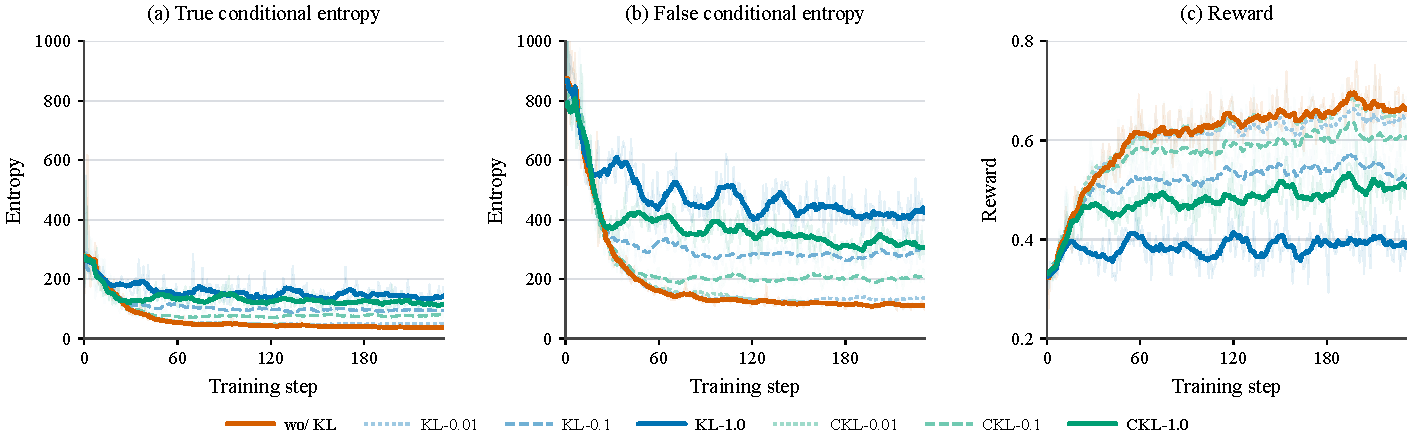
\includegraphics[width=\linewidth]{media/conditional_kl_comparison.pdf}
  \caption{The comparison of KL and Conditional KL (CKL) regularization in RL. We trained Qwen3-1.7B-Base~\citep{yang_qwen3_2025} on MATH~\citep{hendrycks_measuring_2021} dataset with GRPO~\citep{shao_deepseekmath_2024} algorithm and different KL penalities. Two conditional entropies are measured on the sequence level. We can see that strong KL control strength severely limits the reward increment in RL, while CKL regularization allows the model to obtain higher reward while maintaining the diversity of true samples.}
  \label{fig:kl-ckl-comparison}
\end{figure}

\begin{figure}[!htb]
  \centering
  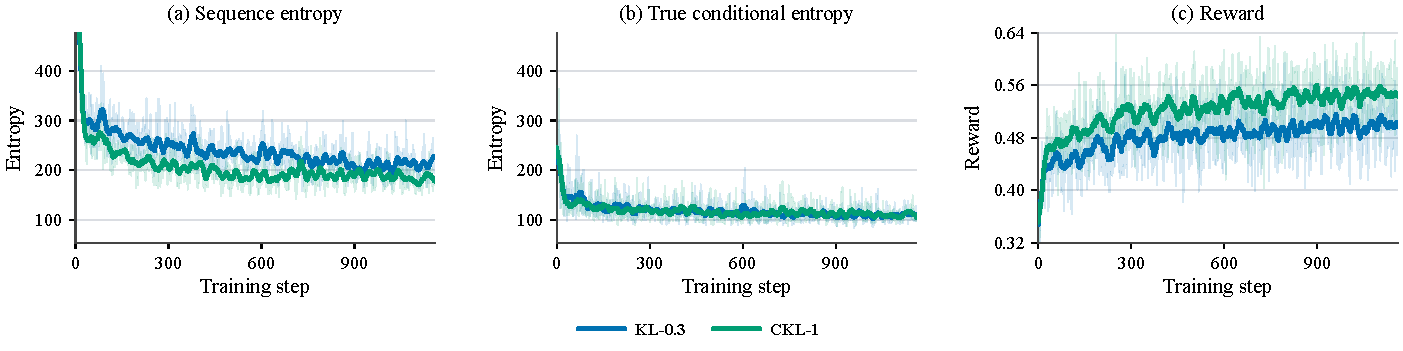
\includegraphics[width=\linewidth]{media/extended_conditional_kl_comparison.pdf}
  \caption{Extended experiments on KL and CKL regularization. These experiments follows the same setting as that in Figure~\ref{fig:kl-ckl-comparison}. We can see that CKL-1 and KL-0.3 exhibits similar regularization ability on conditional distribution, while CKL-1 constantly obtains higher accuracy. Its entropy will thus be slightly lower according to the accuracy-weighted decomposition.}
  \label{fig:ext-ckl-cmp}
\end{figure}

As shown in Figure~\ref{fig:kl-ckl-comparison}, we indeed observe that CKL effectively relaxes the constraint imposed by standard KL regularization on accuracy improvements while preserving the true conditional entropy. Although CKL cannot achieve completely lossless regularization due to cross-sequence interactions induced by model parameterization, it nevertheless demonstrates substantial practical value.

% We also evaluated these models on various test sets. As we can see in Figure~\ref{fig:passk-eval}, although on certain datasets such as Apex2025, the pass@k performance of the base model still surpasses the CKL regularized RL model, CKL still exhibit weaker collapse with higher accuracy compared with standard KL under the same control strength.

This advantage of CKL still holds for up to 20 training epochs, as shown in Figure~\ref{fig:ext-ckl-cmp}. We then evaluated these models on different math datasets, where CKL regularization did exhibit higher performance and generalizability over KL of similar strength, See Figure~\ref{fig:passk-eval}. More related results could be found in Section~\ref{app:rl-exps}.

\begin{figure}[!htb]
  \centering
  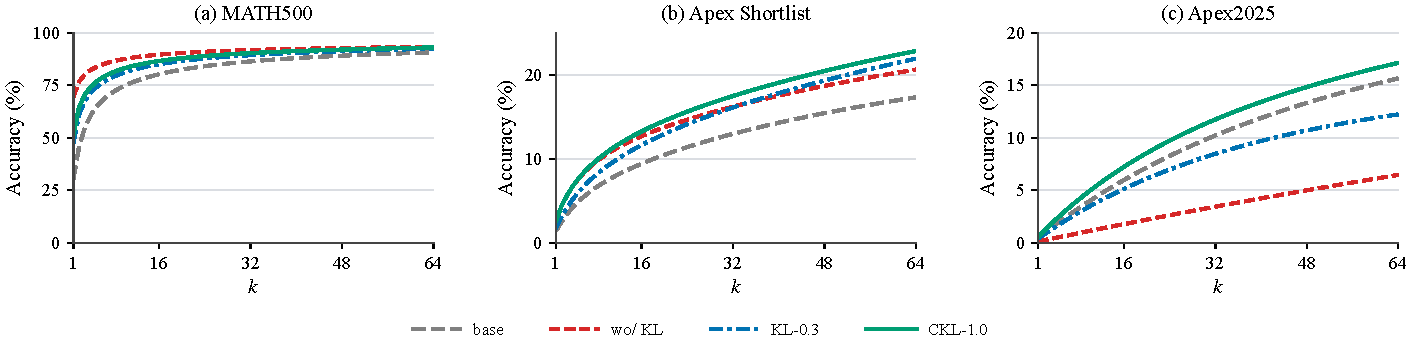
\includegraphics[width=\linewidth]{media/passk_comparison_epoch20.pdf}
  \caption{The comparison of pass@k performance on MATH500~\citep{lightman_lets_2023}, Apex Shortlist~\citep{balunovic_matharena_2025} and Apex2025~\citep{balunovic_matharena_2025}. Models are trained for 20 epochs on MATH dataset. We can see that models trained without KL has higher accuracy on datasets similar to the training set, while severe collapse occurs on harder datasets like Apex2025. CKL constantly achieves higher generalizability over KL regularization across these experiments.}
  \label{fig:passk-eval}
\end{figure}

% We characterize this term for one SGD update of a frozen-feature softmax readout at a fixed prefix $s$. Write $p_i=\pi_{W_0}(i\mid s)$ and $\varepsilon=\eta\|\phi(s)\|_2^2$. For a token subset $\mathcal S$ with equal expected advantage $A_i=a>0$, let $P_{\mathcal S}=\sum_{i\in\mathcal S}p_i$ and $q_i=p_i/P_{\mathcal S}$. With deterministic binary token rewards, $\mathcal S$ can be the success set, so $q$ is the true conditional target and $a=1-P_{\mathcal S}$.
%
% \begin{lemma}[First-order concentration under REINFORCE]
% \label{lem:rl-conditional-drift}
% Under this setup, a REINFORCE update gives
% \begin{equation}
%  \mathbb E[\Delta q_i]
%  =\varepsilon aP_{\mathcal S}q_i(q_i-M_2)+O(\varepsilon^2),
%  \qquad M_2=\sum_{j\in\mathcal S}q_j^2.
%  \label{eq:rl-conditional-drift}
% \end{equation}
% Tokens with $q_i>M_2$ gain conditional probability at first order. The first-order change in $H(q)$ is strictly negative unless $q$ is uniform, despite all tokens in $\mathcal S$ having equal expected advantage.
% \end{lemma}
% \noindent\hyperref[app:dynamics-reinforce]{Proof: Appendix~\ref*{app:dynamics-reinforce}, Lemma~\ref*{lem:dyn-reinforce}.}
%
% Related difficulties arise in classical RL, where policies can stall near suboptimal solutions. Log-barrier regularization helps maintain updates to low-probability actions and hence preserves the diversity~\citep{agarwal_theory_2020}. Under the same readout model, adding an inverse-probability correction with a constant signal cancels the first-order drift within $\mathcal S$.
%
% \begin{lemma}[First-order drift cancellation under normed-ls]
% \label{lem:rl-drift-cancellation}
% Under the same setup, adding the detached correction $a/(Vp_Y)$ to the sampled advantage in the REINFORCE loss gives normed-ls, where $V$ is the vocabulary size. This cancels the first-order expected drift of both the conditional distribution and its entropy:
% \begin{equation}
%  \mathbb E[\Delta q_i]=O(\varepsilon^2),
%  \qquad \mathbb E[\Delta H(q)]=O(\varepsilon^2).
%  \label{eq:rl-drift-cancellation}
% \end{equation}
% \end{lemma}
% \noindent\hyperref[app:dynamics-normed-ls]{Proof: Appendix~\ref*{app:dynamics-normed-ls}, Lemma~\ref*{lem:dyn-normed-ls}.}
%
% Note that this cancellation concerns the first-order mean drift; finite-step sampling noise can still change the conditional distribution and its entropy. The strict cancellation requires accurate estimation of per-token advantage, which is generally inaccessible in practice. So in the following experiments we used a simplified version of normed-ls method, using a constant to replace the advantage weight in the theoretical implementation. It already exhibits certain advantage over GRPO and MaxRL in experiments, while its performance equipped with a value model remains to be explored.

% TODO Experiments of normed-ls


\section{Limitation}

In the previous sections we proposed a framework that unifies different training algorithms via distribution matching objective. For RL algorithms we only analyzed the simplest 0-1 binary reward setting. For more generalized multi-value reward RL we can also extend the distribution matching by introducing a randomized acceptance event, see Appendix~\ref{app:conditional-kl-maxrl}. However, a detailed investigation of its properties is left for future work.

A more important limitation of this work is that, we did not consider generalization ability of these methods. The main theoretical results derived in this paper apply directly to the behavior on the training set, while a more complete understanding of the corresponding behavior on the test set requires further theoretical analysis. Nevertheless, many of our experiments are also conducted on the test set, where we empirically observe behavior similar to that on the training set.

% TODO link to empirical results on the test set


\section{Conclusions}

Distribution matching offers a new perspective on LLM training algorithms. The objective of a variety of LLM training algorithms can be unified as a divergence between the policy model and a target distribution. The target distribution itself also serves as an effective lens through which the properties of training algorithms can be analyzed.

In this work, we show that forward KL distribution matching exhibits non-vanishing variance in the proximal limit, which provides a possible explanation for the advantage of OPD over SFT in proximal settings. Furthermore, for iterative algorithms such as RL, we find that the cumulative effect of this non-vanishing variance can lead to entropy collapse of the target distribution. This observation offers a potential explanation for the degradation of output diversity observed under prolonged RL training in related studies. Motivated by the role of the target distribution in RL, we further develop a Conditional KL regularization method and empirically demonstrate its advantages over classical KL regularization in language model. We hope that our findings can provide useful insights for future research and practical applications in this area.

% In this work, by conducting a variance analysis under specific forms of the target distribution, we provide a theoretical characterization of the regimes in which OPD and SFT are respectively effective.
%
% When the target distribution depends on the model itself, on the other hand, certain forms of performance degradation in the training process can be naturally attributed to the drift of the target distribution. We establish and empirically validate a phenomenon in which the accumulation of optimization variance leads to a progressive decrease in the entropy of the target distribution, providing a possible explanation for degradation phenomena observed in reinforcement learning.
%
% Furthermore, when the RL gradient remains nonzero, analyzing the drift of the target distribution can also suggest principled and reliable correction mechanisms. We believe that our theoretical framework and the associated results can be extended to the study of a broader class of training algorithms and provide useful insights for future research.


\bibliography{ce}
\bibliographystyle{iclr2027_conference}

\clearpage
\appendix
\numberwithin{equation}{section}
\section{Related Works}

Modern LLM training typically begins with pretraining on massive datasets, with the goal of modeling the natural language distribution and acquiring broad world knowledge. Mid-training generally follows the same underlying learning paradigm, while differences in training data and parameter configurations can lead to substantially different outcomes. In the post-training stage, a common practice is to train specialized expert models for tasks in different domains, typically using SFT for cold start followed by task-specific RL algorithms. These expert models can then be distilled into a unified model through methods such as OPD, resulting in a final general-purpose model~\citep{deepseek-ai_deepseek-v4_2026, team_kimi_2026, glm-5-team_glm-5_2026}.

\subsection{Distribution Matching Perspective}

Among the algorithms used across different stages of LLM training, most admit a relatively clear interpretation from the perspective of distribution matching, with RL being a notable exception. Despite its distinctive optimization formulation, RL has also been widely recognized as closely related to distribution matching~\citep{korbak_reinforcement_2022}. Prior to our work, a number of studies investigated the connection between RL and distribution-matching objectives and derived locally optimal solutions with an exponential-tilting form similar to that in our Theorem~\ref{lem:reward-reweighting}~\citep{korbak_rl_2022, korbak_reinforcement_2022}. Reward-induced conditional distributions have likewise been studied in prior work and have motivated several algorithmic improvements~\citep{tajwar_maximum_2026, zhou_variational_2025}.

In most previous studies, however, such distributions primarily appeared as auxiliary results in the derivation or analysis of RL objectives. Subtle discrepancies remain between RL optimization and direct distribution matching, preventing the two perspectives from being fully unified~\citep{korbak_reinforcement_2022}. Recent studies on MaxRL provide an important step toward bridging this gap, revealing a first-order approximation between RL and distribution matching. More importantly, our work differs in that we treat the target distribution induced by distribution matching as a central object of study, rather than merely an intermediate analytical construct. In particular, we study both its role in estimating the training objective and its stochastic evolution throughout training, which together constitute the main results of this work. We expect that this perspective may provide a useful lens for further understanding and improving related training algorithms.

\subsection{Entropy Collapse in RL}

Diversity collapse and entropy decrement in reinforcement learning have long been recognized in the classical RL literature. RL optimization can drive a model toward a suboptimal solution with reduced behavioral diversity, thereby limiting the model's long-term training potential. Classical approaches to mitigating this issue include entropy regularization~\citep{ahmed_understanding_2019} and constraints based on KL divergence~\citep{schulman_trust_2017}. These methods, however, introduce their own trade-offs, including optimization instability and restrictions on reward improvement.

As RL has become increasingly prevalent in LLM post-training, a growing body of work has revisited entropy collapse in this setting. Existing studies have investigated its causes and potential remedies from a variety of perspectives, including biases introduced by PPO clipping~\citep{yu_dapo_2025, cai_beyond_2026, jin_revisiting_2026}, geometric biases induced by model architecture~\citep{ren_learning_2025}, and the underlying training dynamics~\citep{wang_entropy_2026}. In contrast, our analysis identifies a long-horizon degradation of the target distribution caused by variance accumulation. This phenomenon arises at a more fundamental level and does not depend on a particular RL algorithm or implementation trick. Based on this analysis, we further derive a effective regularization strategy. Entropy collapse may represent one of the central challenges in scaling post-training, and our results provide an additional perspective on its underlying mechanism.

\subsection{Variance Control and Training Stability}

The stability of RL algorithms has been studied extensively, with the high variance of training-objective estimators being one of the primary challenges. A substantial fraction of algorithmic developments in RL can be understood as attempts to address this issue~\citep{konda_onactor-critic_2003, schulman_trust_2017, schulman_proximal_2017}. Advantage estimation is among the most widely adopted approaches: it can be implemented using a separate critic model~\citep{konda_onactor-critic_2003, schulman_trust_2017, schulman_proximal_2017}, or approximated through techniques such as group-based sampling and normalization~\citep{shao_deepseekmath_2024, ahmadian_back_2024}. Beyond advantage estimation, the treatment of importance weights and the design of the underlying training infrastructure can also have a substantial impact on optimization stability~\citep{zheng_group_2025, gao_soft_2025}.

Recent empirical evidence suggests that, in the LLM setting, the strong prior induced by extensive pretraining can enable stable RL training over a meaningful range even in the absence of aggressive variance-reduction techniques~\citep{ahmadian_back_2024}. Nevertheless, controlling training variance can still yield measurable performance gains. Our analysis further provides a possible explanation for these gains: reducing training variance not only stabilizes individual optimization steps, but can also mitigate the degradation of the training target caused by variance accumulation over time. As a result, the model is more likely to preserve meaningful exploration and reach better regions of the parameter space.

\section{Proof of Reward Reweighting Under a Forward-KL Restriction}
\label{app:reward-reweighting}

\begin{insight}
The forward-KL penalty makes the optimum interior and unique, so a single
Lagrange multiplier determines how each response probability is reweighted.
Responses with the same reward receive the same multiplier, which cancels
when conditioning on a reward level set.
\end{insight}

Fix a prompt $x$ and a finite response space. Write
$p_y=\pi_\theta(y\mid x)>0$, $r_y=r(x,y)\in\mathbb R$, and $\beta>0$.

\begin{proof}[Proof of Theorem~\ref{lem:reward-reweighting}]
On the probability simplex,
\begin{equation}
 F(q)=\sum_yq_yr_y-\beta D_{\mathrm{KL}}(p\Vert q)
 \label{eq:app-reward-forward-objective}
\end{equation}
has Hessian $-\beta\operatorname{diag}(p_y/q_y^2)\prec0$ and tends
to $-\infty$ at the boundary. Its unique maximizer is interior, with
Lagrange conditions
\begin{equation}
 r_y+\frac{\beta p_y}{q_y}-\lambda_x=0
 \quad\Longrightarrow\quad
 q_y^*=\frac{\beta p_y}{\lambda_x-r_y},\qquad
 \sum_y\frac{\beta p_y}{\lambda_x-r_y}=1.
 \label{eq:app-reward-forward-stationarity}
\end{equation}
The normalization sum decreases continuously from $+\infty$ to $0$
on $(\max_y r_y,\infty)$, determining a unique $\lambda_x$.
For any nonempty $\mathcal S_a=\{y:r_y=a\}$,
\begin{equation}
 q^*(y\mid\mathcal S_a)
 =\frac{p_y\beta/(\lambda_x-a)}
        {\sum_{z\in\mathcal S_a}p_z\beta/(\lambda_x-a)}
 =p(y\mid\mathcal S_a),\qquad y\in\mathcal S_a.
 \label{eq:app-reward-conditional-invariance}
\end{equation}
\end{proof}

\paragraph{Binary rewards.}
For $r_y\in\{0,1\}$ and $0<\rho_\theta(x)<1$, the same solution is
\begin{equation}
 q_y^*=\frac{p_y e^{\alpha_xr_y}}
 {1-\rho_\theta(x)+\rho_\theta(x)e^{\alpha_x}},
 \qquad \alpha_x=\log\frac{\lambda_x}{\lambda_x-1}>0.
 \label{eq:app-reward-binary-tilt}
\end{equation}
Thus $q^*(\mathcal S_1)>\rho_\theta(x)$ and $(q^*)^+=\pi_\theta^+$.
For constant rewards, $q^*=p$.

\paragraph{KL constraint.}
Set $\delta_\beta=D_{\mathrm{KL}}(p\Vert q^*)$.
For any $q$ with $D_{\mathrm{KL}}(p\Vert q)\le\delta_\beta$, optimality gives
\begin{equation}
 \mathbb E_q[r]\le\mathbb E_{q^*}[r]
 +\beta\bigl(D_{\mathrm{KL}}(p\Vert q)-\delta_\beta\bigr)
 \le\mathbb E_{q^*}[r],
 \label{eq:app-reward-constrained}
\end{equation}
with equality only at $q=q^*$.

\section{Proof of the True Conditional KL Identity and Its MaxRL Connection}
\label{app:conditional-kl-maxrl}

\begin{insight}
Conditioning on success rescales every successful response by the same
factor, so the KL reduces to the negative logarithm of the success probability.
Differentiating this probability and using the score identity then gives
the success-weighted MaxRL gradient.
\end{insight}

Let $\mathcal D$ be a fixed empirical prompt distribution. For each $x$,
assume a finite response space, a differentiable positive policy
$\pi_\theta$, and a fixed binary reward. Write
$\mathcal S_x^+=\{y:r(x,y)=1\}$ and assume $\rho_\theta(x)>0$.

\begin{proof}[Proof of Theorem~\ref{lem:conditional-kl-maxrl}]
Since $\pi_\theta^+(y\mid x)=\pi_\theta(y\mid x)/\rho_\theta(x)$ on
$\mathcal S_x^+$ and vanishes elsewhere,
\begin{equation}
 D_{\mathrm{KL}}(\pi_\theta^+\Vert\pi_\theta)
 =\sum_{y\in\mathcal S_x^+}\pi_\theta^+(y\mid x)
       \log\frac1{\rho_\theta(x)}
 =-\log\rho_\theta(x).
 \label{eq:app-success-kl}
\end{equation}
Taking the negative expectation over $x$ proves
Eq.~\eqref{eq:conditional-kl-maxrl}. Moreover,
\begin{equation}
 \nabla_\theta\log\rho_\theta(x)
 =\frac{\sum_y r(x,y)\nabla_\theta\pi_\theta(y\mid x)}{\rho_\theta(x)}
 =\mathbb E_{y\sim\pi_\theta^+(\cdot\mid x)}
       [\nabla_\theta\log\pi_\theta(y\mid x)],
 \label{eq:app-success-score}
\end{equation}
and hence
\begin{equation}
 \nabla_\theta\mathcal J_{\mathrm{MaxRL}}^{(\infty)}
 =\mathbb E_{x\sim\mathcal D,y\sim\pi_\theta(\cdot\mid x)}
 \left[\frac{r(x,y)}{\rho_\theta(x)}
              \nabla_\theta\log\pi_\theta(y\mid x)\right].
 \label{eq:maxrl-gradient}
\end{equation}
\end{proof}

\paragraph{Frozen target.}
For $q_x=\pi_{\theta_0}^+(\cdot\mid x)$,
\begin{equation}
 D_{\mathrm{KL}}(q_x\Vert\pi_\theta)
 =D_{\mathrm{KL}}(q_x\Vert\pi_\theta^+)-\log\rho_\theta(x).
 \label{eq:app-success-frozen-decomposition}
\end{equation}
The first term has zero gradient at $\theta_0$, so
\begin{equation}
 \left.-\nabla_\theta\mathbb E_{x\sim\mathcal D}
 D_{\mathrm{KL}}(q_x\Vert\pi_\theta)\right|_{\theta_0}
 =\left.\nabla_\theta\mathcal J_{\mathrm{MaxRL}}^{(\infty)}
 \right|_{\theta_0}.
 \label{eq:app-success-frozen-gradient}
\end{equation}

\paragraph{Finite-order MaxRL.}
Using $\log\rho=-\sum_{k\ge1}(1-\rho)^k/k$ for $0<\rho\le1$, the
order-$K$ objective of \citet{tajwar_maximum_2026} satisfies
\begin{align}
 \mathcal J_{\mathrm{MaxRL}}^{(K)}
 &=-\mathbb E_{x\sim\mathcal D}
       \left[\sum_{k=1}^{K}\frac{(1-\rho_\theta(x))^k}{k}\right],
 \label{eq:app-maxrl-truncation}\\
 \nabla_\theta\mathcal J_{\mathrm{MaxRL}}^{(K)}
 &=\mathbb E_{x\sim\mathcal D}
       \left[\frac{1-(1-\rho_\theta(x))^K}{\rho_\theta(x)}
                         \nabla_\theta\rho_\theta(x)\right].
 \label{eq:app-maxrl-truncated-gradient}
\end{align}
The geometric sum gives the gradient, and $1/k\le1/(K+1)$ for $k>K$ gives
\begin{equation}
 0\le\mathcal J_{\mathrm{MaxRL}}^{(K)}
             -\mathcal J_{\mathrm{MaxRL}}^{(\infty)}
 \le\mathbb E_{x\sim\mathcal D}
       \left[\frac{(1-\rho_\theta(x))^{K+1}}
                    {(K+1)\rho_\theta(x)}\right].
 \label{eq:app-maxrl-truncation-error}
\end{equation}
Thus $\mathcal J_{\mathrm{MaxRL}}^{(1)}=\mathcal J_{\mathrm{RL}}-1$.
Finite prompt support and $\rho_\theta(x)>0$ imply convergence of the
objective and gradient to Eqs.~\eqref{eq:conditional-kl-maxrl}
and~\eqref{eq:maxrl-gradient} as $K\to\infty$.

\subsection{Extension to Nonbinary Rewards via Randomized Acceptance}
\label{app:randomized-reward-extension}

\begin{insight}
Rescaling a bounded reward to $[0,1]$ allows it to serve as an acceptance
probability. Conditioning on acceptance extends the MaxRL identity to
the joint response--acceptance distribution; standard RL is recovered
at first order.
\end{insight}

Under the same policy assumptions, let the fixed reward satisfy
$a\le r(x,y)\le b$, with constants $a<b$, and set
$s(x,y)=(r(x,y)-a)/(b-a)$.
Introduce $A\mid x,Y\sim\operatorname{Bernoulli}(s(x,Y))$, with kernel
$K_s(1\mid x,y)=s(x,y)$, $K_s(0\mid x,y)=1-s(x,y)$. Define
\begin{equation}
 P_\theta(y,A\mid x)=\pi_\theta(y\mid x)K_s(A\mid x,y),
 \qquad
 \rho_\theta^s(x)=P_\theta(A=1\mid x)
 =\mathbb E_{\pi_\theta(\cdot\mid x)}[s(x,Y)].
 \label{eq:app-randomized-joint}
\end{equation}
Assume $\rho_\theta^s(x)>0$ and condition on $A=1$:
\begin{equation}
 Q_\theta(y,A\mid x)
 =P_\theta(y,A\mid x,A=1)
 =\frac{\pi_\theta(y\mid x)s(x,y)}{\rho_\theta^s(x)}
   \mathbf1\{A=1\}.
 \label{eq:app-randomized-target}
\end{equation}
Since $Q_\theta/P_\theta=1/\rho_\theta^s(x)$ on the support of $Q_\theta$,
\begin{equation}
 -\mathbb E_{x\sim\mathcal D}
 D_{\mathrm{KL}}\bigl(Q_\theta(\cdot,\cdot\mid x)
                 \Vert P_\theta(\cdot,\cdot\mid x)\bigr)
 =\mathbb E_{x\sim\mathcal D}
   \left[\log\mathbb E_{\pi_\theta(\cdot\mid x)}[s(x,Y)]\right].
 \label{eq:app-randomized-kl}
\end{equation}
For the response marginal
$q_\theta^s(y\mid x)=\pi_\theta(y\mid x)s(x,y)/\rho_\theta^s(x)$,
the KL chain rule gives
\begin{equation}
 D_{\mathrm{KL}}(Q_\theta\Vert P_\theta)
 =D_{\mathrm{KL}}(q_\theta^s\Vert\pi_\theta)
  +\mathbb E_{q_\theta^s}[-\log s(x,Y)].
 \label{eq:app-randomized-marginal-kl}
\end{equation}
The expectation is over $s(x,y)>0$. For binary $r$ with $s=r$,
the extra term vanishes, recovering Eq.~\eqref{eq:conditional-kl-maxrl}.
Finally, $\log\rho=(\rho-1)+O((1-\rho)^2)$ near $\rho=1$ gives
standard RL on $s$ at first order, and
$\mathbb E[s]=(\mathbb E[r]-a)/(b-a)$.

\begin{table}[!htbp]
\centering
\caption[Distribution matching for bounded nonbinary rewards]{Continuation
of Table~\ref{tab:distribution-matching}: bounded nonbinary rewards.
Objectives are averaged over prompts $x\sim\mathcal D$. The model distribution is $P_\theta$; the target
$Q_\theta$ conditions it on acceptance and has $Q_\theta(y,0\mid x)=0$.
$^{\dagger}$\,RL is its first-order approximation.}
\label{tab:distribution-matching-nonbinary}
\vspace{5pt}
\begingroup
\small
\setlength{\tabcolsep}{5pt}
\renewcommand{\arraystretch}{1.45}
\begin{tabularx}{\linewidth}{
 >{\raggedright\arraybackslash}p{0.13\linewidth}
 >{\centering\arraybackslash}X
 >{\centering\arraybackslash}p{0.235\linewidth}
 >{\raggedright\arraybackslash}p{0.16\linewidth}}
\specialrule{\heavyrulewidth}{0pt}{0pt}
\rowcolor{frameworktint}
\textcolor{frameworkink}{\textbf{Algorithm}} &
\textcolor{frameworkink}{\textbf{Objective function}} &
\textcolor{frameworkink}{\textbf{Target distribution}} &
\textcolor{frameworkink}{\textbf{Divergence}} \\
\algorithmgroup{Iterative algorithms}
RL &
$\mathbb E_{\pi_\theta}[s(x,Y)]=\rho_\theta^s(x)$ &
$\begin{gathered}
 Q_\theta(y,1\mid x)\\
 =\dfrac{s(x,y)\targetpolicy(y\mid x)}{\rho_\theta^s(x)}
\end{gathered}$ &
\forwardKL$^{\dagger}$ \\
\addlinespace[4pt]
MaxRL (extended) &
$\begin{gathered}
 \log\mathbb E_{\pi_\theta}[s(x,Y)]\\
 =-D_{\mathrm{KL}}(Q_\theta\Vert P_\theta)
\end{gathered}$ &
$\begin{gathered}
 Q_\theta(y,1\mid x)\\
 =\dfrac{s(x,y)\targetpolicy(y\mid x)}{\rho_\theta^s(x)}
\end{gathered}$ &
\forwardKL \\
\bottomrule
\end{tabularx}
\endgroup
\end{table}
\FloatBarrier

\section{Proof of Gradient Noise at the Proximal Limit}
\label{app:proximal-gradient-noise}

\begin{insight}
When student and teacher coincide, every OPD log-ratio weight is zero,
whereas the sampled KD scores cancel only in expectation.
\end{insight}

Fix a prompt $x$, a finite response space, and a fixed positive teacher
$\pi_t$. Let $\pi_\theta>0$ be continuously differentiable near
$\theta_0$, with $\pi_{\theta_0}=\pi_t$.
Write $s_\theta(y\mid x)=\nabla_\theta\log\pi_\theta(y\mid x)$ and
$w_\theta(y\mid x)=\log[\pi_t(y\mid x)/\pi_\theta(y\mid x)]$.
For $m\ge1$, define the sampled-response estimators
\begin{align}
 \widehat g_{\mathrm{KD}}(\theta)
 &=\frac1m\sum_{i=1}^m s_\theta(Y_i\mid x),
 &Y_i&\overset{\mathrm{iid}}{\sim}\pi_t(\cdot\mid x),
 \label{eq:proximal-kd-estimator}\\
 \widehat g_{\mathrm{OPD}}(\theta)
 &=\frac1m\sum_{i=1}^m w_\theta(\widetilde Y_i\mid x)
                          s_\theta(\widetilde Y_i\mid x),
 &\widetilde Y_i&\overset{\mathrm{iid}}{\sim}\pi_\theta(\cdot\mid x).
 \label{eq:proximal-opd-estimator}
\end{align}

\begin{proof}[Proof of Lemma~\ref{lem:proximal-gradient-noise}]
Since $\mathbb E_{\pi_\theta}[s_\theta]=\nabla_\theta\sum_y\pi_\theta(y\mid x)=0$,
\begin{align}
 \nabla_\theta[-D_{\mathrm{KL}}(\pi_t\Vert\pi_\theta)]
 &=\mathbb E_{\pi_t}[s_\theta],
 \label{eq:proximal-kd-gradient}\\
 \nabla_\theta[-D_{\mathrm{KL}}(\pi_\theta\Vert\pi_t)]
 &=\mathbb E_{\pi_\theta}[(w_\theta-1)s_\theta]
 =\mathbb E_{\pi_\theta}[w_\theta s_\theta],
 \label{eq:proximal-opd-gradient}
\end{align}
so both estimators are unbiased. At $\theta_0$, $w_{\theta_0}=0$ and
$\mathbb E_{\pi_t}[s_{\theta_0}]=0$. Therefore
$\widehat g_{\mathrm{OPD}}(\theta_0)=0$ almost surely, while independence gives
\begin{equation}
 \operatorname{Cov}(\widehat g_{\mathrm{KD}}(\theta_0))
 =\frac1m\mathbb E_{\pi_t}[s_{\theta_0}s_{\theta_0}^{\top}]
 =\frac1m F_x(\theta_0).
 \label{eq:app-proximal-fisher}
\end{equation}
For $A\in\{\mathrm{KD},\mathrm{OPD}\}$, set
$V_A(\theta)=\mathbb E\|\widehat g_A(\theta)
-\mathbb E\widehat g_A(\theta)\|_2^2$.
Then
\begin{align}
 mV_{\mathrm{KD}}(\theta)
 &=\mathbb E_{\pi_t}\|s_\theta\|_2^2
       -\|\mathbb E_{\pi_t}s_\theta\|_2^2,\nonumber\\
 mV_{\mathrm{OPD}}(\theta)
 &=\mathbb E_{\pi_\theta}[w_\theta^2\|s_\theta\|_2^2]
       -\|\mathbb E_{\pi_\theta}[w_\theta s_\theta]\|_2^2.
 \label{eq:proximal-estimation-error}
\end{align}
These finite sums are continuous in $\theta$. If
$\operatorname{Tr}F_x(\theta_0)>0$, then
$V_{\mathrm{OPD}}(\theta_0)=0<V_{\mathrm{KD}}(\theta_0)$, so the strict
inequality persists in a neighborhood of $\theta_0$.
\end{proof}

\section{A Conditional Variance Comparison in the Distal Regime}
\label{app:distal-gradient-variance}

\begin{insight}
Suppressing teacher probability on a set still sampled by the student
introduces a growing $\log(1/\epsilon)$ term in the OPD weights.
Separating this term from a bounded remainder reveals quadratic growth
of OPD variance under the stated nonzero-score condition, while KD variance
remains bounded by the fixed student scores.
\end{insight}

Fix $x$, a finite response space $\mathcal Y_x$, and a positive policy
$\pi_\theta$ continuously differentiable near $\bar\theta$. Write
$p_y=\pi_{\bar\theta}(y\mid x)$ and
$s_y=\nabla_\theta\log\pi_\theta(y\mid x)|_{\bar\theta}$.
For a nonempty proper subset $\mathcal A$ of $\mathcal Y_x$, set
$a=\sum_{y\in\mathcal A}p_y\in(0,1)$. Given fixed positive distributions
$u$ on $\mathcal A$ and $v$ on its complement, define
\begin{equation}
 \pi_{t,\epsilon}(y\mid x)=
 \begin{cases}
   \epsilon u_y,&y\in\mathcal A,\\
   (1-\epsilon)v_y,&y\notin\mathcal A,
 \end{cases}
 \qquad 0<\epsilon<1.
 \label{eq:distal-teacher-family}
\end{equation}
With $m$ independent responses and teacher $\pi_{t,\epsilon}$, let
$V_A(\epsilon)=\operatorname{Tr}\operatorname{Cov}(\widehat g_A(\bar\theta))$
for the estimators in
Eqs.~\eqref{eq:proximal-kd-estimator}--\eqref{eq:proximal-opd-estimator}.

\begin{lemma}[Variance amplification under teacher-probability suppression]
\label{lem:distal-gradient-variance}
If $\sum_{y\in\mathcal A}p_y\|s_y\|_2^2>0$, then, as $\epsilon\to0$,
\begin{equation}
 V_{\mathrm{OPD}}(\epsilon)
 =\frac{C_{\mathcal A}}m\log^2\frac1\epsilon
       +O\!\left(\frac{\log(1/\epsilon)}m\right),
 \qquad V_{\mathrm{KD}}(\epsilon)\le\frac{G^2}{m},
 \label{eq:distal-variance-growth}
\end{equation}
where $G=\max_y\|s_y\|_2$ and
\begin{equation}
 C_{\mathcal A}
 =\sum_{y\in\mathcal A}p_y\|s_y\|_2^2
       -\left\|\sum_{y\in\mathcal A}p_ys_y\right\|_2^2>0.
 \label{eq:distal-variance-coefficient}
\end{equation}
Consequently, for every fixed $R>0$, sufficiently small $\epsilon$
gives $V_{\mathrm{OPD}}(\epsilon)>R V_{\mathrm{KD}}(\epsilon)$.
\end{lemma}

\begin{proof}
Set $L=\log(1/\epsilon)$ and
$w_\epsilon(y)=\log[\pi_{t,\epsilon}(y\mid x)/p_y]$. Then
\begin{equation}
 w_\epsilon(y)=-L\mathbf1_{\mathcal A}(y)+b_\epsilon(y),
 \qquad
 b_\epsilon(y)=
 \begin{cases}
   \log(u_y/p_y),&y\in\mathcal A,\\
   \log(v_y/p_y)+\log(1-\epsilon),&y\notin\mathcal A.
 \end{cases}
 \label{eq:distal-weight-decomposition}
\end{equation}
For $0<\epsilon\le1/2$, $b_\epsilon$ and $s$ are uniformly bounded.
Expanding the variance under $Y\sim p$ gives
\begin{equation}
 mV_{\mathrm{OPD}}(\epsilon)
 =L^2\operatorname{Tr}\operatorname{Cov}_p
       (\mathbf1_{\mathcal A}(Y)s_Y)+O(L)
 =L^2 C_{\mathcal A}+O(L).
 \label{eq:distal-variance-expansion}
\end{equation}
Cauchy--Schwarz yields
$C_{\mathcal A}\ge(1-a)\sum_{y\in\mathcal A}p_y\|s_y\|_2^2>0$.
For KD,
$mV_{\mathrm{KD}}(\epsilon)
\le\mathbb E_{\pi_{t,\epsilon}}\|s_Y\|_2^2\le G^2$,
which proves Eq.~\eqref{eq:distal-variance-growth} and the comparison
for any fixed $R>0$. Also,
$D_{\mathrm{KL}}(p\Vert\pi_{t,\epsilon})=aL+O(1)\to\infty$.
\end{proof}

\section{Variance Accumulation in Iterative Algorithms}\label{sec:variance-accumulation}

\begin{insight}
  In iterative algorithms, the target distribution helps separate intended gains from unintended side effects. For example, RL aims to maximize expected reward. With binary rewards, conditioning on $r(x,y)=1$ yields the training target $\pi_\theta^+$, which remains unchanged under the ideal update in \hyperref[lem:reward-reweighting]{Theorem~\ref*{lem:reward-reweighting}}. Tracking how this target changes during training can therefore reveal side effects beyond the intended reward improvement.
\end{insight}

Distillation algorithms have a fixed target distribution for the student to fit. Although we have showed in \hyperref[lem:reward-reweighting]{Theorem~\ref*{lem:reward-reweighting}}, the ideal single-step update of RL or MaxRL with binary reward will not affect the target distribution, this property may not hold in real applications. One important reason is that, there are non-negligible random noise in the one optimization step. This could be caused by the empirical estimator of the objective, the approximation of the optimizer and the numerical precision of the model parameter.

In this section we study \emph{variance accumulation} in iterative training and its relation to the observed entropy dynamics, starting from the gradient noise in self-distillation.

\subsection{Iterative Self-Distillation}

We start from \emph{iterative self-distillation}: each step samples responses from the current model and increases their log-likelihood, treating the sampling distribution as fixed during differentiation. This is the uncentered RL update with reward $1$ for every response, and coincides with sampled-response SFT at the proximal limit. The distinction is that, in SFT at the proximal limit, the target distribution is fixed as $\pi_t = \pi_{\theta_0}$, whereas in iterative self-distillation the target distribution is $\displaystyle\targetpolicy$ which updates with the current policy.

%Unlike SFT, the teacher is replaced by the updated student after each step. This is also the common practice adopted by RL algorithms.

By \hyperref[lem:proximal-gradient-noise]{Lemma~\ref*{lem:proximal-gradient-noise}}, the sampled gradient has zero mean but generally nonzero variance. Fix a prompt $x$, write $\pi_k=\pi_{\theta_k}(\cdot\mid x)$, and let $\mathcal F_k$ denote the training history before sampling at step $k$. Then we have the following result:

\begin{lemma}[Martingale structure of self-distillation]
\label{lem:self-distillation-martingale}
For iterative self-distillation with step size $\eta_k$, the parameters form a martingale. The induced probabilities satisfy the same property to first order:
\begin{equation}
 \mathbb E[\theta_{k+1}\mid\mathcal F_k]=\theta_k,
 \qquad
 \mathbb E[\pi_{k+1}(y)\mid\mathcal F_k]
 =\pi_k(y)+O(\eta_k^2).
 \label{eq:self-distillation-martingale}
\end{equation}
\end{lemma}
\noindent\hyperref[app:variance-accumulation]{Proof: Appendix~\ref*{app:variance-accumulation}.}

The martingale property also yields an entropy decrease when entropy is locally concave along the updates.

\begin{theorem}[Conditional decrease of expected entropy]
\label{lem:self-distillation-entropy}
Let $h_x(\theta)=H(\pi_\theta(\cdot\mid x))$. If $h_x$ is concave along every possible update segment from $\theta_k$ to $\theta_{k+1}$, then
\begin{equation}
 \mathbb E[H(\pi_{k+1})\mid\mathcal F_k]\le H(\pi_k).
 \label{eq:self-distillation-entropy}
\end{equation}
The inequality is strict under nonzero conditional update variance. If these conditions hold at each step, expected entropy decreases over training.
\end{theorem}
\noindent\hyperref[app:variance-accumulation]{Proof: Appendix~\ref*{app:variance-accumulation}.}

Thus sampling noise can deterministicly reduce expected entropy even when the parameter update has zero mean, while iterative generation severely amplifies this effect. We should note that the iterative training is unavoidable in RL or self-distillation theoretically, since the distribution drift already occurs, the objective itself will require updating the actor's parameter or introducing importance sampling correction~\citep{schulman_proximal_2017}.

This expectational decrease of entropy should be understood in this way: We have no guarantee on the deterministic direction of entropy in each step. If one training step happens to generate some samples with low probability, self-distillation on these samples will actually increase the sample entropy. So this is not contradictive with previous researches that carefully analyzed the condition when a single learning step will increase or decrease the entropy~\citep{cui_entropy_2025, ren_learning_2025, jin_revisiting_2026, wang_entropy_2026}. This result in fact takes a step further, and answers if we are doing the update multiple times, or in the long-term of training, how should the entropy change on average. The long-term expectation cancels the randomness in a single step update, and gives a deterministic decrement.

% TODO Empirical results on iterative self-distillation

\subsection{Reversed Iterative Self-Distillation}

The empirical results of iterative self-distillation is somehow not very surprising, since we can easily make another explanation: the sequence with higher probability are more likely to be sampled and strengthened, naturally resulting in a sharpened distribution. This is often used to explain the entropy collapse in RL~\citep{cui_entropy_2025, hao_rethinking_2026}. This is an intuitive explanation that treats the entropy collapse as a property of the expectation form RL algorithm rather than empirical variance accumulation.

To further distinguish the potential cause, we designed reversed iterative self-distillation experiments, where these two explanations could give contradictive predictions, and our experiments support the counter-intuitive one.

The reversed iterative self-distillation is achieved by setting all rewards in self-distillation to -1. Hence we are pushing down the probability of every sequence generated by the policy model, and the sequence with higher sample probability will receive more punishment. If we accept the common explanation on the entropy dynamics in LLM training, this would flatten the sample distribution and increase the sample entropy of the policy model.

However, changing the training direction in self-distillation do not affact the zero mean gradient, and hence the martingale property in \hyperref[lem:self-distillation-martingale]{Theorem~\ref*{lem:self-distillation-martingale}} still holds. Then with the same derivation as \hyperref[lem:self-distillation-entropy]{Lemma~\ref*{lem:self-distillation-entropy}}, the variance accumulation will also guatantee a decrement of sample entropy in expectation.

% TODO Empirical results on reversed iterative self-distillation

\section{Proof of the Accuracy-Weighted Entropy Decomposition}
\label{app:rl-target-entropy}

Fix a prompt $x$, a finite response space, and a deterministic binary reward.
Write $\rho=\rho_\theta(x)\in(0,1)$,
$p=\pi_\theta(\cdot\mid x)$, and $p^\pm=\pi_\theta^\pm(\cdot\mid x)$.
Then
\begin{equation}
 p^+(y)=\frac{r(x,y)p(y)}{\rho},
 \qquad
 p^-(y)=\frac{(1-r(x,y))p(y)}{1-\rho}.
 \label{eq:rl-success-failure-distributions}
\end{equation}

\begin{proof}[Proof of Lemma~\ref{lem:rl-target-entropy}]
Since $p^+$ and $p^-$ have disjoint supports and
$p=\rho p^++(1-\rho)p^-$, using $0\log0=0$ gives
\begin{align*}
 H(p)
 &=-\rho\sum_y p^+(y)\log\bigl(\rho p^+(y)\bigr)
   -(1-\rho)\sum_y p^-(y)\log\bigl((1-\rho)p^-(y)\bigr)\\
 &=h_{\mathrm b}(\rho)+\rho H(p^+)+(1-\rho)H(p^-),
\end{align*}
which proves Eq.~\eqref{eq:rl-entropy-decomposition}.
For fixed $p^+$ and $p^-$ with $H(p^+)<H(p^-)$,
\begin{equation*}
 \frac{\mathrm d}{\mathrm d\rho}
 \bigl[\rho H(p^+)+(1-\rho)H(p^-)\bigr]
 =H(p^+)-H(p^-)<0.
\end{equation*}
\end{proof}

\section{Proof of the Conditional KL Estimator}
\label{app:ckl-estimator}

\begin{insight}
On successful responses, the sequence log-ratio is the sum of a
success-probability log-ratio and a conditional-distribution log-ratio.
Centering within successes removes the former exactly. Multiplying the
remaining signal by the policy score gives the conditional-KL gradient.
Using the same samples to estimate the mean introduces a finite-group
scaling factor, with zero signal for groups containing fewer than two successes.
\end{insight}

Fix a prompt $x$ and a finite response space with a deterministic binary
reward and a nonempty success set $\mathcal S^+$.
Write $p_\theta=\pi_\theta(\cdot\mid x)$, $p=p_{\theta_0}$,
$q=\pi_{\mathrm{ref}}(\cdot\mid x)$, $\rho_\theta=p_\theta(\mathcal S^+)$,
$\rho=\rho_{\theta_0}$, and $\rho_q=q(\mathcal S^+)$.
Assume $p_\theta$ is differentiable and both $p_\theta$ and $q$ are positive.
Superscript $+$ denotes conditioning on $\mathcal S^+$;
all gradients below are evaluated at $\theta_0$.

\begin{proof}[Proof of Theorem~\ref{thm:ckl-estimator}]
Let $d(y)=\log(p(y)/q(y))$, $\mu=\mathbb E_{p^+}[d(Y)]$, and
$K(\theta)=D_{\mathrm{KL}}(p_\theta^+\Vert q^+)$.
For $y\in\mathcal S^+$,
\begin{equation}
 d(y)=\log\frac{\rho}{\rho_q}+\log\frac{p^+(y)}{q^+(y)},
 \qquad
 d(y)-\mu=\log\frac{p^+(y)}{q^+(y)}-K(\theta_0).
 \label{eq:ckl-log-ratio-decomposition}
\end{equation}
The scores $s=\nabla\log p_\theta$ and $s^+=\nabla\log p_\theta^+$ satisfy
$s=s^++\nabla\log\rho_\theta$ on $\mathcal S^+$ and
$\mathbb E_{p^+}[s^+]=0$. Hence
\begin{align}
 \nabla K
 &=\mathbb E_{p^+}\!\left[
 s^+(Y)\left(\log\frac{p^+(Y)}{q^+(Y)}+1\right)\right]\notag\\
 &=\mathbb E_{p^+}[s^+(Y)(d(Y)-\mu)]
  =\mathbb E_{p^+}[s(Y)(d(Y)-\mu)].
 \label{eq:ckl-conditional-gradient}
\end{align}

Conditional on $N=n\ge2$, relabel the successful responses as
$Y_1,\ldots,Y_n\overset{\mathrm{iid}}{\sim}p^+$.
Set $\bar d=n^{-1}\sum_{j=1}^n d(Y_j)$,
$a=\mathbb E_{p^+}[d(Y)s(Y)]$, and $b=\mathbb E_{p^+}[s(Y)]$.
Independence gives
\begin{align}
 \mathbb E[\bar d\,s(Y_i)\mid N=n]
 &=\frac{a}{n}+\frac{n-1}{n}\mu b,\notag\\
 \mathbb E[(d(Y_i)-\bar d)s(Y_i)\mid N=n]
 &=\frac{n-1}{n}(a-\mu b)
  =\frac{n-1}{n}\nabla K.
 \label{eq:ckl-sample-centering-factor}
\end{align}
Summing over the $n$ successes and dividing by $G$ proves
Eq.~\eqref{eq:ckl-finite-gradient}; for $n\le1$, both sides are zero.
Multiplication by $-\beta$ gives the stated expected gradient contribution.
Finally, $(d_i+a_0)-(\bar d+a_0)=d_i-\bar d$ proves invariance
under a common shift of the successful log-ratios.
\end{proof}

% \input{appendices/token_learning_dynamics}

\section{Supplementary Experiments on Proximal and Distal Distillation}
\label{app:distillation-experiments}

We provide the experimental settings and additional results for the
distillation comparison in the main body. The experiments consider three
settings: a teacher identical to the initial student, teachers obtained
by briefly training the initial student with GRPO, and an existing strong
teacher applied to students with different initial capabilities. These
settings allow us to examine the proximal-limit prediction and the
behavior of distillation beyond this limit.

\subsection{Experimental settings}

\paragraph{Distillation objectives.}
Let $\pi_\theta$ be the student and $\pi_t$ a frozen teacher. Following
the main body, the two population objectives to maximize are
\begin{align}
 \mathcal J_{\mathrm{KD}}(\theta)
 &=-\mathbb E_{x\sim\mathcal D}
 D_{\mathrm{KL}}\bigl(\pi_t(\cdot\mid x)\Vert
                       \pi_\theta(\cdot\mid x)\bigr),
 \label{eq:app-distillation-kd}\\
 \mathcal J_{\mathrm{OPD}}(\theta)
 &=-\mathbb E_{x\sim\mathcal D}
 D_{\mathrm{KL}}\bigl(\pi_\theta(\cdot\mid x)\Vert
                       \pi_t(\cdot\mid x)\bigr).
 \label{eq:app-distillation-opd}
\end{align}
Sampled-response KD approximates the teacher expectation using a fixed
cache $\mathcal C_t$ of prompt--response pairs. Its empirical loss is
\begin{equation}
 \widehat{\mathcal L}_{\mathrm{SFT}}(\theta)
 =-\frac{1}{|\mathcal C_t|}\sum_{(x,y)\in\mathcal C_t}
   \sum_{k=1}^{|y|}\log\pi_\theta(y_k\mid x,y_{<k}).
 \label{eq:app-distillation-sft-loss}
\end{equation}
This is the SFT implementation of KD referred to in the figures and
tables. OPD instead samples from the current student and obtains
teacher log-probabilities on the student's prefixes. Writing
\begin{equation}
 w_\theta(y\mid x)
 =\log\frac{\pi_t(y\mid x)}{\pi_\theta(y\mid x)}
 =\sum_{k=1}^{|y|}\log
   \frac{\pi_t(y_k\mid x,y_{<k})}{\pi_\theta(y_k\mid x,y_{<k})},
 \label{eq:app-distillation-log-ratio}
\end{equation}
the corresponding population gradient is
\begin{equation}
 \nabla_\theta\mathcal J_{\mathrm{OPD}}
 =\mathbb E_{x\sim\mathcal D,\,y\sim\pi_\theta(\cdot\mid x)}
 \left[w_\theta(y\mid x)\nabla_\theta\log\pi_\theta(y\mid x)\right].
 \label{eq:app-distillation-opd-gradient}
\end{equation}
The sampled responses and log-ratio weights are detached in the score
update, as in Appendix~\ref{app:proximal-gradient-noise}. Thus both
methods match the same teacher distribution, but use different sampling
distributions and gradient weights. Task rewards only monitor response
correctness and do not contribute to either distillation objective.

\paragraph{Models and training.}
For the proximal-limit experiment, we initialize both the student and
the frozen teacher from Qwen3-1.7B-Base. For the proximal experiments,
we use the same initial student and three GRPO-trained teachers,
denoted GRPO-50, GRPO-100, and GRPO-200. For the remaining experiments,
we use a JustRL teacher with R1-Distill-1.5B and Qwen2.5-Math-1.5B
students. Both students use the same cached teacher responses for SFT.
The latter pair has a larger initial benchmark performance gap.

Training uses the slime framework with Megatron and SGLang, at revision
\texttt{a067ce6f}. The Qwen3 experiments use DAPO17k, a maximum response
length of 2,048 tokens. The JustRL experiments use the JustRL training
data and a maximum response length of 8,192 tokens. Runs use seed 1.
The proximal-limit runs use a learning rate of $10^{-5}$.

\paragraph{Evaluation and interpretation of the curves.}
Each evaluation samples 16 responses per problem at temperature 1,
with a maximum response length of 16,384 tokens, and uses the
DAPO/math-verify grader. Scores are average correctness over sampled
responses, expressed as percentages. We evaluate on AIME-2024, AMC23,
and MATH500 and report their unweighted mean.

The reward curves have different meanings for the two methods. For
OPD, they measure correctness of responses generated by the evolving
student. For SFT, they measure correctness of the cached teacher
responses in each batch. The SFT curves can therefore fluctuate with
batch composition even though the response cache is fixed. Their level
does not measure the trained student's performance. We use the separate
held-out evaluations for comparisons between the two methods.
The recorded Qwen3 base reference uses a shorter evaluation limit of
4,096 tokens.

\subsection{Behavior at the proximal limit}

Figure~\ref{fig:distillation-proximal-limit} shows gradient norms when
the frozen teacher initially coincides with the student. In addition to
offline SFT on a fixed self-generated cache, we include online SFT,
which refreshes responses from the current student, and controls that
reverse the update direction. In the legend, ``fwd'' and ``rev'' denote
the ordinary and sign-reversed updates, respectively; they do not denote
the two directions of KL divergence.

\begin{figure}[htbp]
\centering
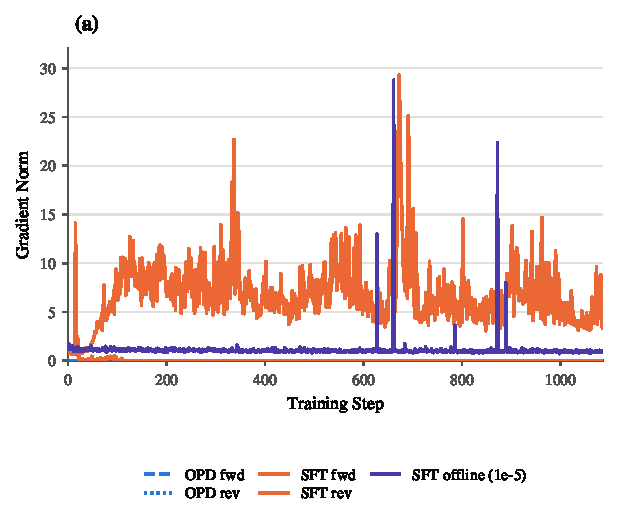
\includegraphics[width=0.68\linewidth]{media/selfdist_gradnorm.pdf}
\caption{Gradient norms with Qwen3-1.7B-Base as both the initial student
and the frozen teacher. Both OPD directions have zero recorded gradient
norm throughout training, with their traces overlapping at zero.
The SFT runs exhibit nonzero sampled gradients. Offline SFT uses a
fixed cache, whereas the other SFT controls regenerate responses from
the evolving student. All runs use a learning rate of $10^{-5}$.}
\label{fig:distillation-proximal-limit}
\end{figure}

Both OPD runs have exactly zero recorded gradient norm throughout
training. This agrees with Lemma~\ref{lem:proximal-gradient-noise}:
the sampled log-ratio weight vanishes when teacher and student coincide,
so reversing its sign also leaves the update zero. SFT exhibits nonzero
sampled gradients even at initialization, as expected for sampled-response
cross-entropy. Offline SFT subsequently fits the finite response cache,
while online SFT also changes its sampling distribution as training
proceeds. Thus the initial contrast illustrates the proximal-limit
prediction; the later SFT trajectory is no longer a measurement at that
limit. In particular, a training gradient norm is not a direct estimate
of gradient variance at fixed parameters.

\begin{takeaway}
At the proximal limit, both distillation objectives have zero population
gradient, but their sampled updates behave differently: OPD vanishes
samplewise while sampled-response KD retains gradient noise. This
illustrates the gradient-estimation distinction underlying the proximal
advantage discussed in the main body.
\end{takeaway}
\FloatBarrier

\subsection{Distillation from nearby teachers}

Figure~\ref{fig:distillation-proximal} shows training with the three
GRPO teachers. Student rollout correctness under OPD quickly
approaches the range of the corresponding teacher-cache correctness.
The evaluations in Table~\ref{tab:distillation-performance}
provide the student-to-student comparison. OPD attains
mean scores of 17.77, 20.75, and 26.63 for GRPO-50, GRPO-100, and
GRPO-200, compared with 16.78, 19.81, and 26.07 for SFT.
These observations are consistent with a local advantage of
OPD, although the single-seed results do not establish statistical
significance or directly test the gradient-variance ordering.
%
% \begin{figure}[htbp]
% \centering
% 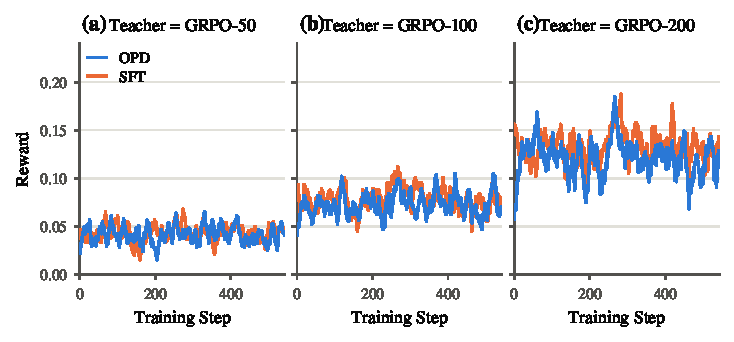
\includegraphics[width=\linewidth]{media/selfdist_proximal.pdf}
% \caption{Distillation from the three GRPO-trained Qwen3 teachers.
% OPD rewards measure current student rollout correctness; SFT rewards
% measure cached teacher-response correctness, rather than SFT student
% performance. Each panel uses Qwen3-1.7B-Base as the initial student.}
% \label{fig:distillation-proximal}
% \end{figure}

\FloatBarrier

\subsection{Distillation with a larger initial performance gap}

Figure~\ref{fig:distillation-distal} compares two students trained
with the JustRL teacher. The R1-Distill-1.5B student starts at a mean
benchmark score of 53.56, compared with 72.27 for the teacher. Both
methods reach scores close to the teacher: SFT and OPD scores
are 72.94 and 72.04, respectively. Under this setting both algorithms remain stable, while SFT is already slightly more performant.

The Qwen2.5-Math-1.5B student starts substantially lower, at 15.27.
Its OPD rollout correctness decreases early and remains low over the
displayed interval, whereas SFT reaches an evaluation score of
47.46.

\begin{figure}[htbp]
\centering
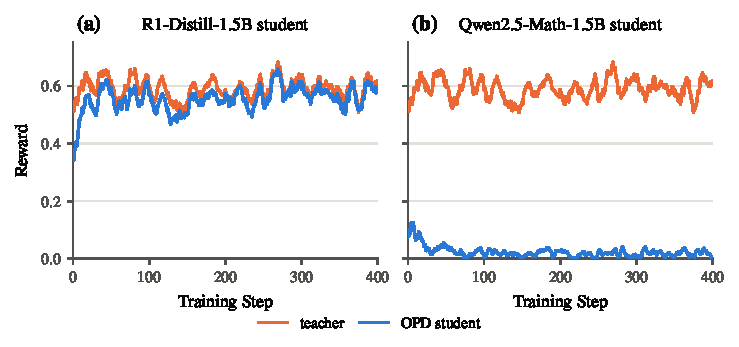
\includegraphics[width=\linewidth]{media/selfdist_distal.pdf}
\caption{Reward curve of distal OPD with the JustRL teacher and two initial students.
OPD rollout correctness increases for R1-Distill-1.5B but decreases
and remains low for Qwen2.5-Math-1.5B. Note that since we do not have student's on policy samples in SFT, we can not draw a similar reward curve for SFT. Their
evaluation results are reported in
Table~\ref{tab:distillation-performance}.}
\label{fig:distillation-distal}
\end{figure}

These results illustrate that successful OPD depends on the
teacher--student pair. They are compatible with the conditional
variance comparison in Appendix~\ref{app:distal-gradient-variance},
but do not identify gradient variance as the cause of the observed
failure. The experiments change the student initialization and do not
measure the teacher-probability suppression condition in
Lemma~\ref{lem:distal-gradient-variance}. Consequently, they do not
establish that a large performance gap alone implies OPD instability.
\FloatBarrier

\clearpage
\subsection{Evaluation results}

\begin{table}[htbp]
\centering
\caption{Evaluation results of OPD and SFT with 16 sampled responses per problem. We can see that OPD typically outperforms SFT in proximal distillation, while it may experience severe instability issue in distal distillation.}
\label{tab:distillation-performance}
\vspace{5pt}
\begingroup
\small
\setlength{\tabcolsep}{5pt}
\renewcommand{\arraystretch}{1.45}
% Match the main table's group headings, spanning all seven columns here.
\newcommand{\distillationgroup}[1]{%
  \specialrule{\lightrulewidth}{2pt}{0pt}%
  \multicolumn{7}{l}{\textcolor{frameworkink}{\textbf{#1}}}\\%
  \specialrule{\lightrulewidth}{0pt}{2pt}}
% Account for the partial rule when vertically centering each four-row cell.
\newcommand{\distillationcell}[2]{%
  \multirow[c]{4}{#1}[-\dimexpr(\aboverulesep+\belowrulesep+\cmidrulewidth)/2\relax]{#2}}
% Shift Teacher left by transferring 8pt of width from Student to its right padding.
  \begin{tabularx}{\linewidth}{>{\raggedright\arraybackslash}X l<{\hspace{14pt}} l r r r r}
\specialrule{\heavyrulewidth}{0pt}{0pt}
\rowcolor{frameworktint}
\textcolor{frameworkink}{\textbf{Student}} &
\textcolor{frameworkink}{\textbf{Teacher}} &
\textcolor{frameworkink}{\textbf{Model}} &
\textcolor{frameworkink}{\textbf{AIME-24}} &
\textcolor{frameworkink}{\textbf{AMC23}} &
\textcolor{frameworkink}{\textbf{MATH500}} &
\textcolor{frameworkink}{\textbf{Mean}} \\
\distillationgroup{Proximal Distillation}
\distillationcell{=}{Qwen3-1.7B-Base} & \distillationcell{*}{GRPO-50} & Student & 0.62 & 7.50 & 16.19 & 8.10 \\
 & & Teacher & 1.04 & 12.19 & 25.62 & 12.95 \\
\cmidrule(l){3-7}
 & & SFT & \textbf{1.88} & \underline{15.78} & \underline{32.69} & \underline{16.78} \\
 & & OPD & \underline{1.25} & \textbf{16.25} & \textbf{35.80} & \textbf{17.77} \\
\midrule
\distillationcell{=}{Qwen3-1.7B-Base} & \distillationcell{*}{GRPO-100} & Student & 0.62 & 7.50 & 16.19 & 8.10 \\
 & & Teacher & \textbf{1.67} & \underline{18.28} & 33.50 & 17.82 \\
\cmidrule(l){3-7}
 & & SFT & \underline{1.04} & \textbf{19.06} & \underline{39.32} & \underline{19.81} \\
 & & OPD & 0.62 & \textbf{19.06} & \textbf{42.58} & \textbf{20.75} \\
\midrule
\distillationcell{=}{Qwen3-1.7B-Base} & \distillationcell{*}{GRPO-200} & Student & 0.62 & 7.50 & 16.19 & 8.10 \\
 & & Teacher & 2.50 & 22.50 & 46.27 & 23.76 \\
\cmidrule(l){3-7}
 & & SFT & \textbf{3.33} & \underline{25.16} & \underline{49.73} & \underline{26.07} \\
 & & OPD & \underline{2.92} & \textbf{25.62} & \textbf{51.36} & \textbf{26.63} \\
\distillationgroup{Distal Distillation}
\distillationcell{=}{R1-Distilled-Qwen-1.5B} & \distillationcell{*}{JustRL-DS} & Student & 21.04 & 63.75 & 75.90 & 53.56 \\
 & & Teacher & \textbf{49.38} & 83.28 & 84.16 & \underline{72.27} \\
\cmidrule(l){3-7}
 & & SFT & \underline{47.92} & \textbf{85.16} & \textbf{85.74} & \textbf{72.94} \\
 & & OPD & 47.29 & \underline{83.44} & \underline{85.39} & 72.04 \\
\midrule
\distillationcell{=}{Qwen2.5-Math-1.5B} & \distillationcell{*}{JustRL-DS} & Student & 4.38 & 18.44 & 23.00 & 15.27 \\
 & & Teacher & \textbf{49.38} & \textbf{83.28} & \textbf{84.16} & \textbf{72.27} \\
\cmidrule(l){3-7}
 & & SFT & \underline{11.88} & \underline{56.09} & \underline{74.41} & \underline{47.46} \\
 & & OPD & -- & -- & -- & -- \\
\bottomrule
\end{tabularx}
\endgroup
\end{table}

Table~\ref{tab:distillation-performance} shows that OPD achieves a
higher mean score than SFT with each of the three nearby teachers.
For R1-Distill-1.5B, both methods attain performance close to the
JustRL teacher, with SFT obtaining the higher mean score. For
Qwen2.5-Math-1.5B, SFT improves the student's mean score from 15.27
to 47.46, while direct OPD fails. The relative effectiveness of the
two objectives therefore varies across teacher--student pairs.

\begin{takeaway}
OPD is favored in the proximal comparisons, consistent with its
local gradient-estimation advantage, while sampled-response KD remains
effective in the larger-gap setting where direct OPD fails.
\end{takeaway}
\FloatBarrier

\section{Supplimentary Experiments on Standard and Reversed Iterative Self-Distillation}

Here are some supplimentary experiments on two iterative self-distillation methods mentioned in the main body, See Figure~\ref{fig:supp-exp-isd}.

\begin{figure}[htb]
\centering
\includegraphics[width=\linewidth]{media/entropy_comparison_ISD.pdf}
\caption{Additional experiments on entropy dynamics of iterative self-distillation and reversed iterative self-distillation. In the legend ``N'' denotes the number of samples per request, ``B'' denotes batchsize and ``lr'' denotes the learning rate of SGD optimizer.}
\label{fig:supp-exp-isd}
\end{figure}

\begin{takeaway}
In a single training step, model entropy may randomly increase or decrease, but over the long run it exhibits a deterministic downward trend in expectation.
\end{takeaway}

These entropy curves satisfies the derivation in the main body very well. In fact the decreasing expected entropy does not guarantee the probability of decrement and increment. For example in reversed iterative self-distillation, since the punishment on samples with a high probability will raise the entropy, the entropy policy model has a high probability to be increased. However, the negative expectation indicates that once the decrement happens, the magnitude of the decrease will be substantial. This was also observed in our experiments.

These experiments share these experimental settings:

\begin{itemize}
\item seed: 1
\item total\_train\_epochs: 2
\item actor.path: Qwen/Qwen3-1.7B-Base
\item dataset: openai/gsm8k
\item actor.dtype: bfloat16
\item actor.kl\_ctl: 0
\item actor.optimizer.type: sgd
\item actor.optimizer.momentum: 0
\end{itemize}

Other hyperparameters are kept the same as the default value of AReaL, which can be found in our codebase.

\section{Supplimentary Experiments on Reinforcement Learning}

\subsection{Additional Ablation Study on Advantage Estimation}

Here are some other supplimentary experiments on RL absent in the main body. They provide more evidence on the theoretical results obtained by our analysis and beyond.

\begin{figure}[htb]
  \centering
  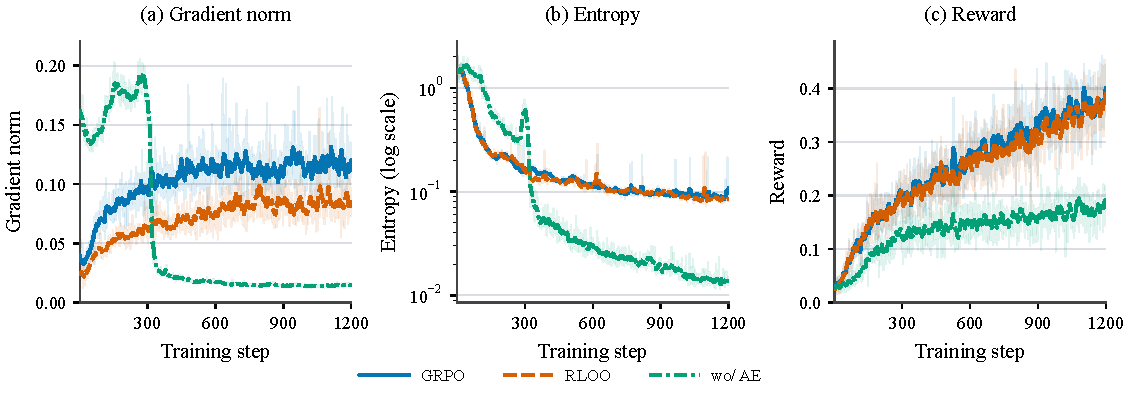
\includegraphics[width=\linewidth]{media/adv_estimators_comparison_smollm.pdf}
  \caption{The ablation study on the advantage estimation on SmolLM2-360M-Instruct~\citep{allal_smollm2_2025} and GSM8K~\citep{cobbe_training_2021} dataset. with batchsize 128, n\-samples 4 and AdamW optimizer with learning rate 1e-5.}
  \label{fig:supp-exp-rl-smollm}
\end{figure}

In Figure~\ref{fig:supp-exp-rl-smollm} we also examined the variance effect on smaller models like SmolLM2-360M-Instruct. We used similar training settings like that in \citet{tajwar_maximum_2026}. We can see that advantage estimation methods effectively prevents entropy collapse and stabilizes the training process. These experiments share the following hyperparameter settings in AReaL~\citep{fu_areal_2025}, unmentioned hyperparameters are kept the same as the default setting:

\begin{itemize}
  \item seed: 1
  \item batchsize: 128
  \item n\_samples: 4
  \item total\_train\_steps: 1200
  \item actor.optimizer.lr: 1e-5
  \item actor.reward\_scaling: 2.0
  \item actor.reward\_bias: -0.5
\end{itemize}

\subsection{Additional Results on Conditional KL Restriction}

\begin{figure}[htb]
  \centering
  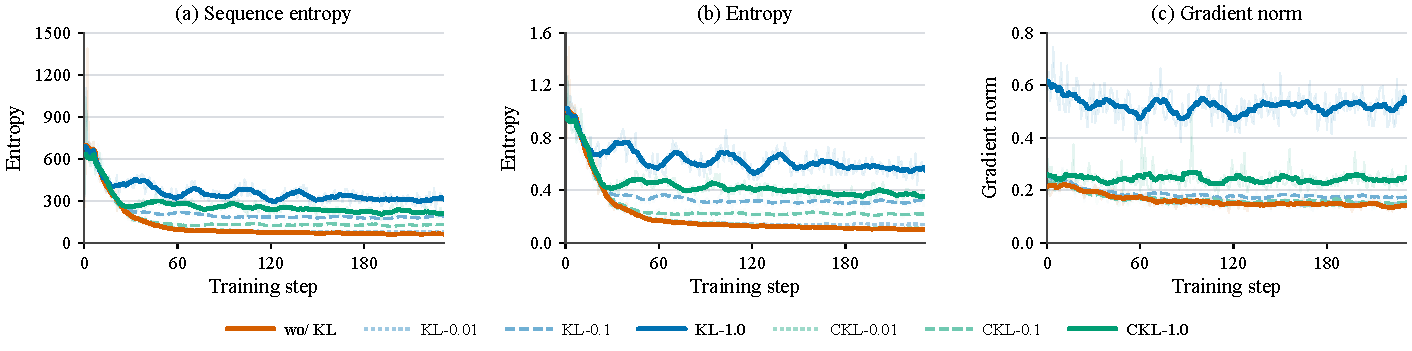
\includegraphics[width=\linewidth]{media/conditional_kl_metrics.pdf}
  \caption{Additional metrics on the comparison of KL and CKL restrictions.}
  \label{fig:addi-kl-ckl}
\end{figure}

The results in Figure~\ref{fig:addi-kl-ckl} come from the same set of experiments as that in Figure~\ref{fig:kl-ckl-comparison}. We can see that the sequence-level entropy showed the same decreasing trend as that of token-level entropy. Recall the entropy decomposition in Lemma~\ref{lem:rl-target-entropy}, the entropy of a model in RL is only comparable if they have similar accuracy. Otherwise the entropy value may not directly reflect the collapse in diversity. The gradient norm behavior of these experiments also provides some explanation on the advantage of CKL restriction. With high restriction strength, the gradient of CKL is much more modest while it still preserves the diversity very well.

These experiments adopts these hyperparameter settings, while unmentioned ones use the default value in AReaL~\citep{fu_areal_2025}:

\begin{itemize}
  \item seed: 1
  \item batchsize: 128
  \item n\_samples: 4
  \item total\_train\_epochs: 4
  \item actor.optimizer.lr: 1e-6
  \item actor.reward\_scaling: 2.0
  \item actor.reward\_bias: -0.5
  \item actor.kl\_estimator: "k1"
\end{itemize}


\begin{figure}[htb]
  \centering
  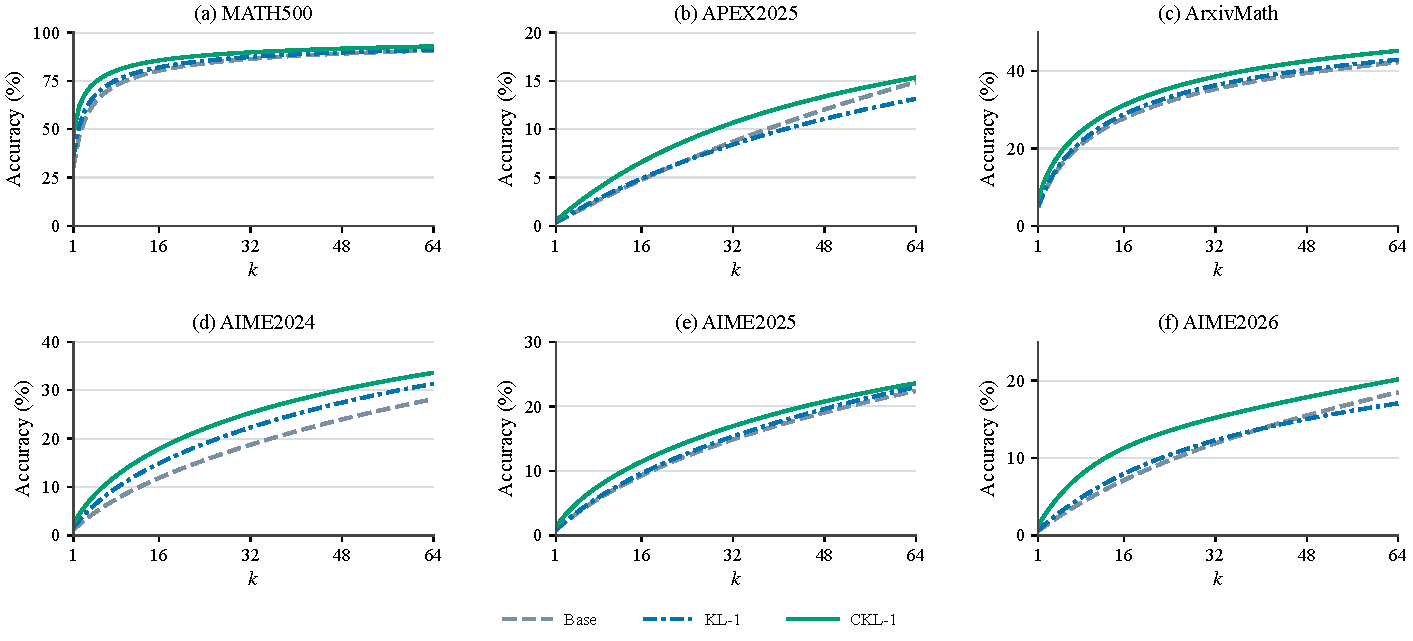
\includegraphics[width=\linewidth]{media/passk_comparison_appendix.pdf}
  \caption{Extended pass@k performance of models trained with KL or CKL regularization. CKL regularization also preserves more learning potential in the sense of pass@k performance compared with KL regularization with the same strength. The evaluation settings is the same as that used in AReaL training pipeline.}
  \label{fig:passk-eval-full}
\end{figure}



\end{document}
